    \documentclass[twoside, english, rapport]{ffiarticle}

    %=============================================================
    % Standard LaTeX mal, kommenter ut linja med 'ffiarticle' og
    % 'ffi_spesifikt' - gj�r livet litt enklere mens du skriver ;-)

    %\documentclass[norsk,twoside,a4paper,12pt]{article}
    %\setlength{\parindent}{0pt}
    %\setlength{\parskip}{1.5ex}
    %\usepackage{times}
    %\usepackage{hyperref}


    %=============================================================
    \usepackage{lmodern}
    \usepackage{graphicx}
    \graphicspath{{figures/}}%Filbaner til dine figurer
    \usepackage{babel}%spr�k
    %\usepackage[T1]{fontenc}%For � kunne skrive �,�,� direkte i *.tex filene
    \usepackage{amsmath,amsbsy,amssymb,amsfonts,alltt,subcaption}%matematikk
    \usepackage[colorlinks]{hyperref}
    \usepackage[capitalize]{cleveref}
    \hypersetup{colorlinks = black,linkcolor=blue}
    \usepackage{multirow}

    %%%%%%%%%
    % Litteraturreferansestiler
    %%%%%%%%%%

    %\usepackage{apacite}
    %\usepackage{harvard} %NB! Husk � bruke en annen bibliografistil enn
    %plain sammen med Harvard-pakka!

    %\usepackage{IEEEtrantools}

    %============================================================
    % Forside
    %============================================================
    %Tittel
    \title{Gas dispersion within an urban street canyon -- a CFD code comparison}
    %Forfatter
    \author{Magnus Aarskaug Rud and Carl Erik Wasberg}

    %Alle FFI spesifikke kommandoer
    %==================================================================
%
%  LaTeX kommandoer for FFI malen (ffiarticle)
%
%==================================================================

%===================================================================
%
% Forside
%
%===================================================================

% Forfatter 
% Settes inn med standard \author{} i hoveddokument
 
% Tittel
% Settes inn med standard \title{} i hoveddokument

% Undertittel 
%\subtitle{ (undertittel) } % Norsk dersom norsk spr�k er valgt, ellers engelsk 

% Engelsk tittel
\englishtitle{(englishtitle)} % Sett inn tekst KUN dersom norsk spr�k er valgt
% NB! dersom engelsk spr�k settes tittel inn med \title{} i hoveddokument 


%====================================================================
%
% Gradering av tittel 
%
%====================================================================

%\unclassifiedtitle % Brukes for � gj�re tittelen ugradert i et gradert dokument
%\restrictedtitle % Brukes for � gj�re tittelen begrenset i et gradert dokument

%====================================================================
%
% Paragrafer i offentlighetsloven. Brukes for dokumenter gradert til
% unntattOffentlighet eller fortrolig 
%
%====================================================================

%\offentlighetsloven{\S5a, jfr forvaltningsloven \S13}

%\offentlighetsloven{\S\ 13 jf fvl \S\ 13}% (Taushetsplikt)}                         
%\offentlighetsloven{\S\ 14}% (Organinterne dokumenter)}                          
%\offentlighetsloven{\S\ 15.1}% (Interne dokumenter utanfr� - underordna organ)}  
%\offentlighetsloven{\S\ 15.2}% (Interne dokumenter utanfr� - r�d og
%vurderingar)}
%\offentlighetsloven{\S\ 20}% (Utanrikspolitiske interesser)}                     
%\offentlighetsloven{\S\ 21}% (Nasjonale forsvars- og tryggingsinteresser)}       
%\offentlighetsloven{\S\ 22 - f�rste punktum}% (Budsjettsaker - departementet)}   
%\offentlighetsloven{\S\ 22 - annet punktum}% Budsjettsaker-                      
                                % underliggende organ                           
%\offentlighetsloven{\S\ 23.1}%�konomi, l�nns- og personalforvaltnign             
%\offentlighetsloven{\S\ 23.3}%Anbud                                              
%\offentlighetsloven{\S\ 25}%Tilsetjingssaker med mer   

%=========================================================================
%
% Nedgraderingstid for et gradert dokument
%
%=========================================================================

%\downgrad{5 YEARS}


%=========================================================================
% 
% Datoer
%
%==========================================================================

\dateofpublishingNo{Dag M�ned �r}
\dateofpublishingEn{\today}

%==========================================================================
%
% Tittelsidas bakside
%
%==========================================================================

% Rapportnummeret
\reportnumber{��rr/yyyyy}

% Prosjektnummer
\projectnumber{xxx}

% ISBN-nummer
%\isbnP{ISBN papirversjon}
%\isbnE{ISBN elektronisk versjon}

% Emneord

\emneord{Neutral gas}
\emneord{Large eddy simulation}
\emneord{Urban street cayon}
\emneord{Fluent performance test}
\emneord{Fluent vs. CDP}
\emneord{Fluent solver settings}

%============================================================================
%
% Sjefer
%
%============================================================================

%Adm. dir.
\directorgeneral{John Mikal St�rdal}
%Avdelingssjef
\divisionmanager{(avdelingssjef)}
%Forskningssjef
%\chiefscientist{(forskningssjef)}
%Prosjektleder
\projectleader{(prosjektleder)}


%============================================================================
% 
% Sammendrag
%
%============================================================================

% Norsk sammendrag

\sammendrag{
Denne rapporten unders�ker hvor godt den kommersielle CFD-programvaren Fluent kan estimere dispersjon 
av n�ytral og tung gass. Testproblemet som er brukt for sammenligning av data
er dispersjon av en n�ytral gass i en vindtunnel med fire kubiske
klosser som representerer et urbant bygningsmilj�.
Resultatene er sammenlignet med data fra et vindtunnel-eksperiment
og tilsvarende simuleringer i CDP\@. Alle simuleringer er utf�rt ved hjelp av Large Eddy Simulations
(LES). Ulike diskretiseringsskjemaer er testet, effekten av en subgrid-scale (SGS) modell
er dokumentert og grunnleggende konvergens egenskaper er bekreftet. 

I byplanlegging og st�rre prosjekter innenfor infrastruktur er det viktig � ha kunnskap til hvordan 
farlige gasser og v�sker b�r behandles. � kunne simulere disse scenarioene tillater oss � v�re 
bedre forberedt p� u�nskede hendelser som gasslekkasje fra en fabrikk. Valg av programvare og 
matematisk formulering er viktig for � kunne tilby en korrekt l�sning innenfor en akseptabel 
tidsramme.

Resultatene fra Fluent stemmer godt overens med de eksperimentelle dataene og simuleringene gjort
i CDP\@. Bredden og h�yden p� gass-skyen som oppst�r som en f�lge av gassutslippet 
er konsistent med tidligere data. Ulike diskretiseringsskjemaer har et signifikant utslag p�
regnetiden og resultatene varierer ogs� i noen grad. 
Selv om tid kan bli spart ved � anvende andre innstillinger enn de som er anbefalt av Fluent, 
tilsier resultatene at standardinstillingene i Fluent gir de mest n�yaktige resultatene.
Simuleringene har v�rt gjennomf�rt p� opptil 120 kjerner og koden kan bekreftes � skalere
sv�rt godt med antall prosesser.
}

% English summary
\abstractdocpage{This report investigates how well the commercial CFD software 
Fluent can estimate gas dispersion of both heavy and neutral gas. 
The reference case used to compare the data is gas dispersion 
of gas in a wind-tunnel with four cubic obstacles representing an urban street canyon. 
The results obtained are compared with data from a wind-tunnel 
experiment and similar simulations performed in CDP\@. All simulations are performed using 
Large Eddy Simulation (LES). Different discretization schemes 
have been tested, the effect of a subgrid-scale model is documented and 
a basic convergence properties are confirmed.

In city planning and large projects within infrastructure it is important to have knowledge of how 
hazardous gases and liquids should be handled. Being able to simulate these scenarios enable us 
to be better prepared for unwanted events such as a factory gas leak. 
The choice of 
software and mathematical formulation helps us provide a correct solution 
within a reasonable amount of time.

The results obtained using Fluent agree well with the experimental data and the CDP simulations, 
The width and height of the plume generated by the gas release is consistent with the previous 
results, but there are some disagreements in the data measured close to the wall.
The choice of discretization scheme has a significant impact on the computational time 
and the results vary to some degree. Allthough the time can be saved by applying a non-default
scheme the results indicate that the default setting in Fluent provides the most accurate solution.
The simulations have been performed on up to 120 cores and the program scales very well as the amount of cores is increased.
}
% Forord
%\forord{Forord er valgfritt}
%Kommenter ut for � bruke standard LaTeX maler
    %===========================================================

    \begin{document}

    \ffititlepage
    % \twocolumn %For tospaltet dokument

    %============================================================
    \section{Introduction}
    %\begin{itemize}
        %\item Description of the problem
        %\item LES - how basic? 
        %\item the wind tunnel experiment and numerical experiment in CDP
        %\item Fluent and CDP
    %\end{itemize}
    The scenario investigated in this work is dispersion of a neutral gas in a rectangular tunnel
    with four cubic blocks placed as obstacles. The blocks have sides $h = 0.109$ m and represent a 
    set of buildings forming a street canyon. The gas is released from a circular source on 
    ground level and
    is translated by the wind field through the canyon, see figure~\ref{fig:layout}.
    In this figure $h$ is used as the length scale. The dotted lines
    indicate the positions where data is collected.
    %
    \begin{figure}[h]
        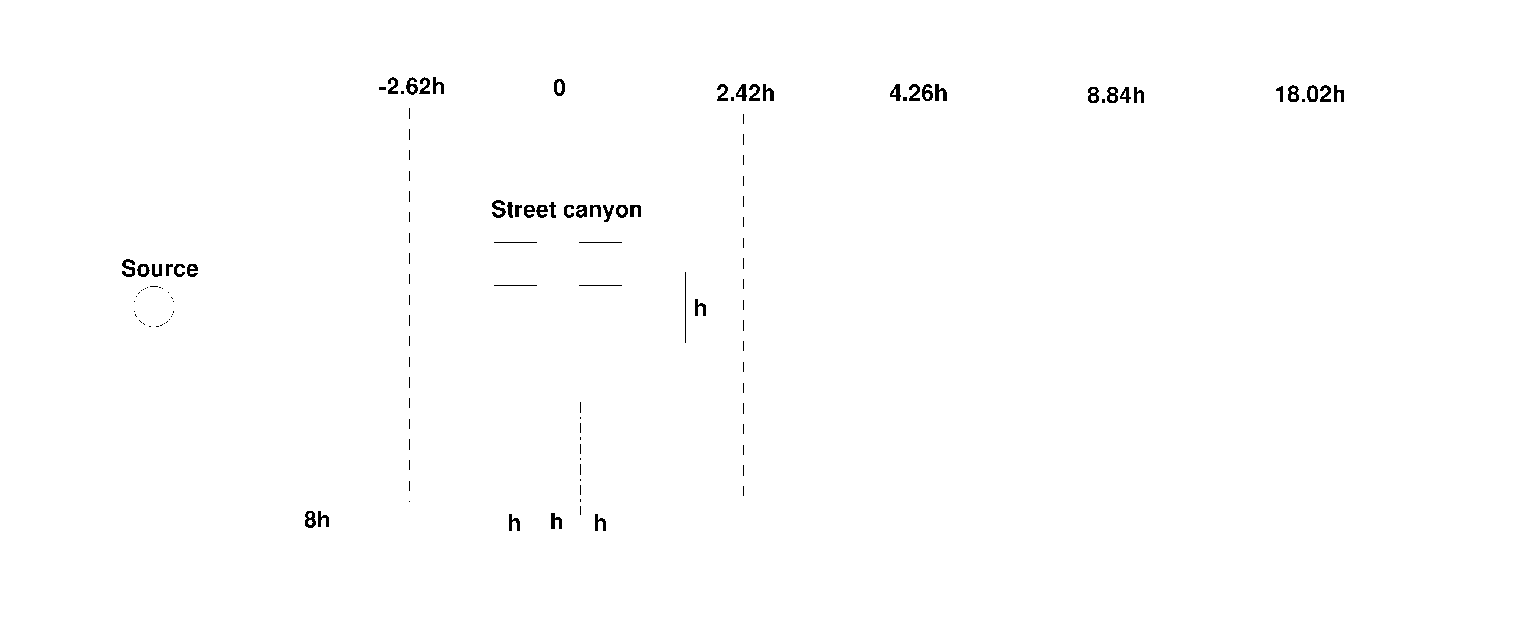
\includegraphics[width=1.1\textwidth]{figures/layout.eps}
        \caption{Schematic overview of the domain from above. The data is collected along the dotted lines.}
    \label{fig:layout}
    \end{figure}
    %

    Scaling the domain with the size of the boundary layer $H =1$ m restricts it to
    the box $1.04\leq x/H \leq 6,-1.75\leq y/H \leq 1.75, 0\leq z/H \leq 1.5$.
    The four cubic boxes are centered around $(2.4715,0)$ with a distance $h$ between each box.
    The source is placed with its center in $(1.436,0)$ and radius $r = 0.0515$.
    The grid used for the simulation consists of $6.2$ million nodes and is described in detail
    in~\cite{eriksson}. It is an unstructured hex-mesh that can be divided into three 
    regions (R1,R2,R3) with different spatial discretization. The finest region is concentrated around the 
    area where the plume is assumed to be located. In addition the grid size defining the source 
    is even finer than in the rest of R1. The grid sizes in wall units, based on the length scale 
    $l^{+}=lU^{*}/\nu$ is specified in table~\ref{tab:gridsize}. The variables $\nu,U^*$ are defined 
    in table~\ref{tab:variables}. An illustration of the three regions 
    is found in figure~\ref{fig:ref}
    \begin{table}[h]
        \centering
        \begin{tabular}{c|c c c|c c c| }
                   &  \multicolumn{3}{|c|}{Scaled grid size} & \multicolumn{3}{|c|}{Grid size in mm}\\
            Region & $\Delta x^+ $ & $\Delta y^+ $ & $\Delta z^+ $ & $\Delta x$  & $\Delta y$  & $\Delta z$ \\ \hline
             Source(R1) & 6.3 & 6.3 & 4.0 - 13 & 1.5 & 1.5 & 1 - 4 \\\hline
             R1         & 13  & 13  & 4.0 - 13 & 4  & 4  & 1 - 4   \\\hline
             R2         & 61  & 61  & 20 - 61  & 13 & 13 & 3 - 17  \\\hline
             R3         & 185 & 185 & 60 - 185 & 45 & 45 & 10 - 50 \\\hline
	\end{tabular}
	\caption{Computational grid size used for the street canyon simulation. $\Delta x^+$ and
	$\Delta y^+$ are constant in each region.}
\label{tab:gridsize}
\end{table}
%
\begin{figure}[h]
	\centering
	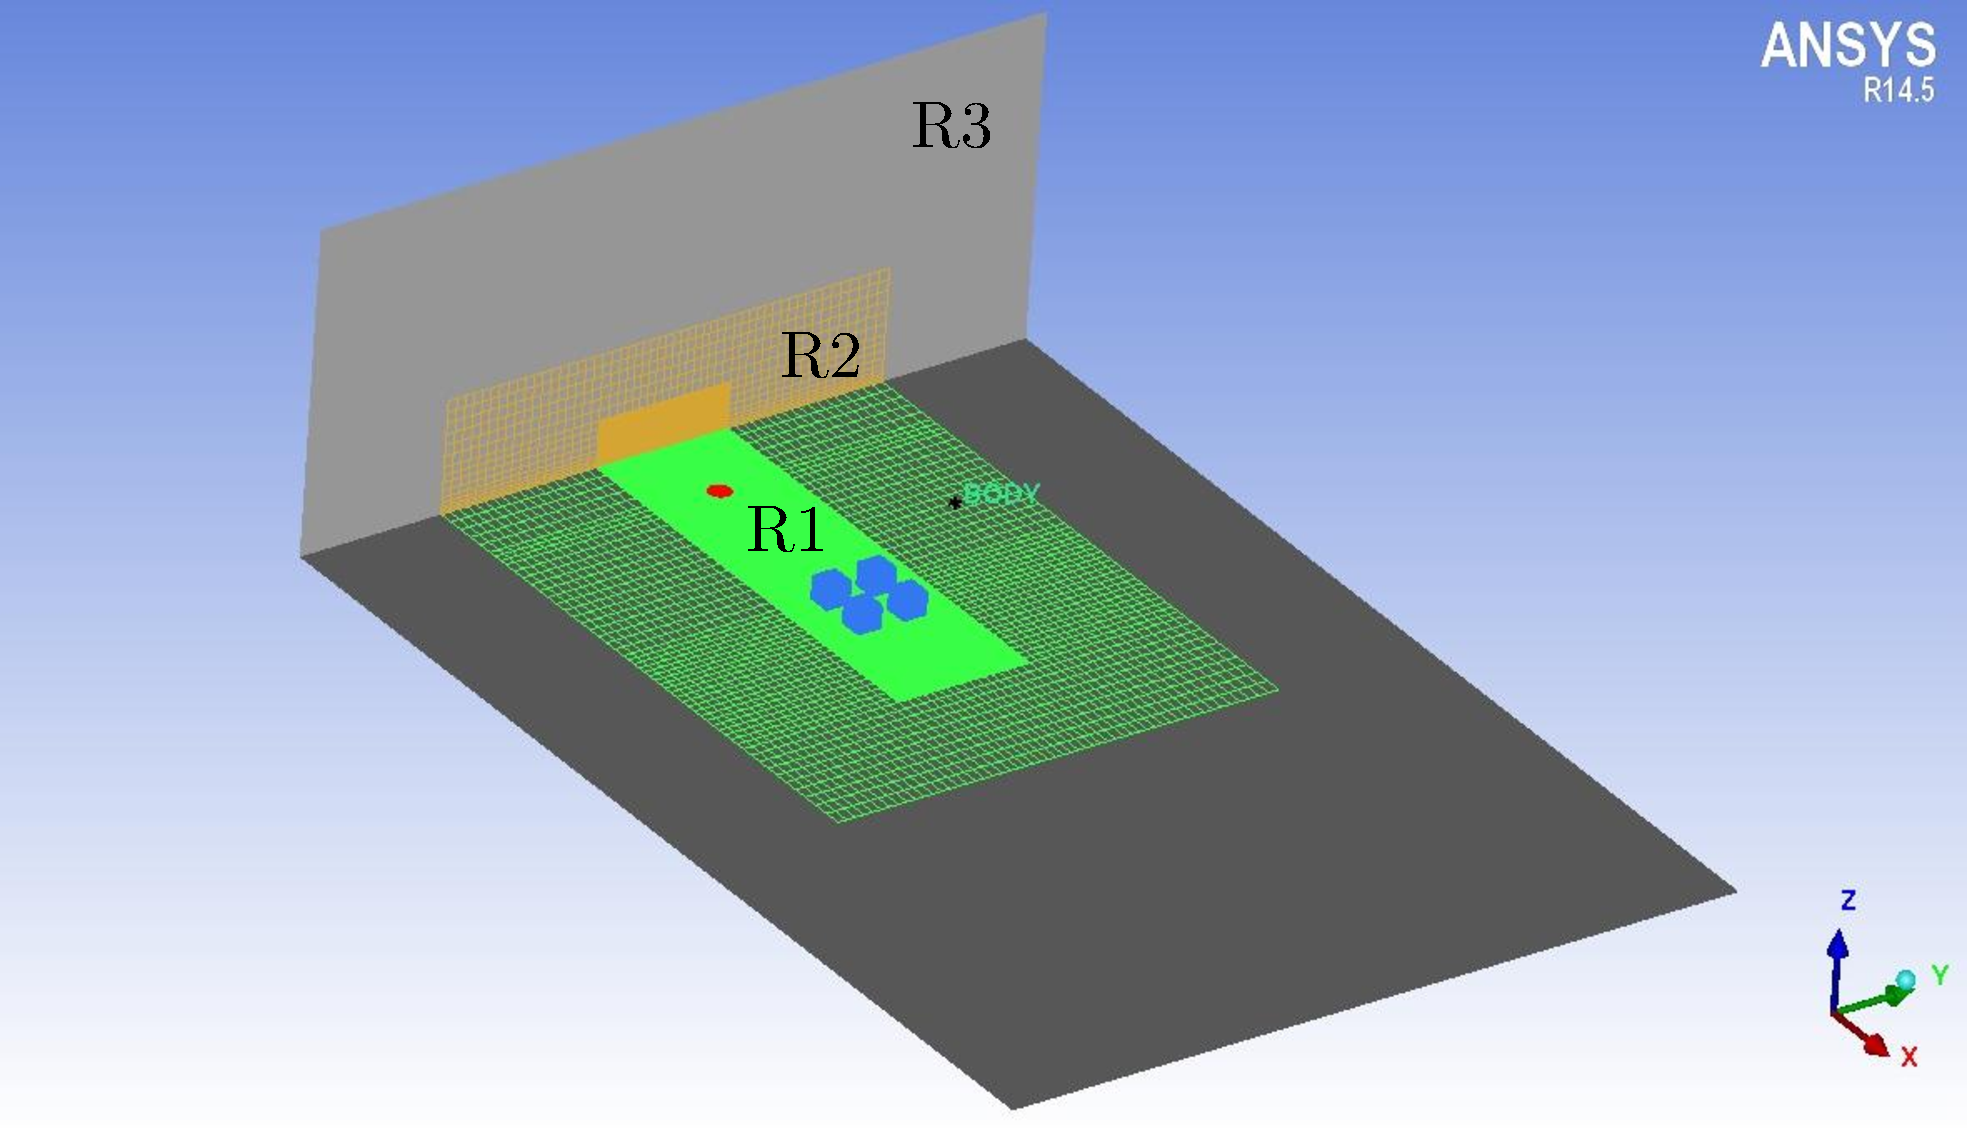
\includegraphics[width=0.9\textwidth]{figures/ref2.pdf}
	\caption{Overview of the three refinement regions}
\label{fig:ref}
\end{figure}
%
The simulations are performed using Large Eddy Simulation (LES) 
with the dynamic Smagorinsky-Lilly subgrid-scale model~\cite{dynsmag}. 
The release of gas will result in a plume that is advected with the wind field. The size and 
shape of the plume at the indicated positions in figure~\ref{fig:layout} are compared with 
experimental data and simulations performed in CDP\@. 
The wind-field in the tunnel is created by an inflow condition that is defined from previous 
simulations in CDP~\cite{eriksson}.
For clarification, some of the variables used a lot throughout this work will be stated explicitly
in table~\ref{tab:variables}.
\begin{table}
    \centering
    \begin{tabular}{c c c c}
        Variable & Value & Unit & Description \\ \hline
        $H$   & $1$ & m & Length scale of the domain \\ 
        $h$   & $0.109$ & m & The sides of the cubic boxes\\ 
        $Q$   & $50$ & dm$^3$/min & Gas release from source \\ 
        $U_{ref}$ & $\approx1.08$ & m/s & Reference value of $U$ \\
        $U^*$ & $\approx 0.06$ & m/s & Friction velocity \\
        $\nu$ & $1.7895\cdot 10^{-5}$& m$^2$/s & Kinematic viscosity \\
    \end{tabular}
    \caption{Essential variables, $U_{ref}$ is calculated as a time average of the velocity in 
        x-direction at a point far away from the floor and walls and will therefore 
        vary by a small amount from case to case. }
\label{tab:variables}
\end{table}

\subsection{CDP vs. Fluent}
	Fluent is a widely used piece of commercial CFD software with many different solvers and 
    discretization schemes available. 
	CDP is a software surging from Stanford University's Center for Integrated Turbulence
	Simulations (CITS), Stanford, California. It is a Finite Volume (FV) based solver 
	specially designed for LES\@. Fluent is also a FV based solver but there are some conceptual 
	differences between the two codes. This section contains a brief introduction into 
	how the numerical solvers are implemented in the two pieces of softwares. 
	
	For the main results in this work, Fluent is used with the default settings 
    for Large Eddy Simulations of viscous incompressible flow with species transport.
	%(Note that the default settings depend on the type of problem about to be solved)
	The algorithm used in Fluent is a pressure-velocity coupling scheme called SIMPLE\@.
	It is a predictor-corrector method for solving the equations of continuity~\cref{eq:continuity}
	and momentum~\cref{eq:momentum} and is documented in the Fluent Theory Guide~\cite{theoryguide}. 
    This scheme provides
	estimations for the velocity $\mathbf{u}$ and the pressure $p$ for each timestep. When these 
	estimations are obtained the transport equation for the species transport is solved. 
	This procedure is continued until convergence is reached within each timestep. 


	The numerical method used in CDP VIDA is a predictor-corrector method 
	developed by Ham (2007)~\cite{Ham} and has a slightly different approach. 
	Instead of first solving for pressure and velocity VIDA makes an initial prediction of 
	the flux and the mass fraction of the species. This allows it to calculate the density. 
	The prediction for flux is then corrected by conserving mass, and the mass fraction is 
	corrected by the transport equation. After doing these calculations the velocity 
	and pressure equations are solved in a coupled manner similar to the way Fluent does it.
	The method is described in \emph{Cascade's User's \& Developer's manual 2014, chap. 9.2}~\cite{CDP}.
	
	The most important 
	difference is that CDP VIDA solves an extra Poisson equation for each iteration and 
  is therefore more stable and achieves faster convergence, whereas the algorithm applied in Fluent 
	requires more iterations per timestep and is more dependent on its stability coefficients.
\section{Mathematical formulation}
Assuming incompressible flow, the governing equations are the continuity equation, 
\begin{align}
	\nabla \cdot \mathbf{u} = 0,
	\label{eq:continuity}
\end{align}
and the Navier-Stokes (N-S) equation obtained by conserving momentum,
\begin{align}
	\rho \frac{\partial \mathbf{u}}{\partial t} + \rho \mathbf{u} \cdot \nabla \mathbf{u} 
	= \rho \mathbf{g} - \nabla p +\frac{\partial}{\partial x_j} 
	\left[ 2\mu S_{ij}
	-\frac{2}{3} \delta_{ij}\frac{\partial u_j}{\partial x_i}\right].
	\label{eq:momentum}
\end{align}
In these equations $\mathbf{u} = [u_1, u_2, u_3]$ is the velocity of the flow, $p$ is the pressure, $\rho$ is the 
mass density of air, $S_{ij}=\frac{1}{2}(\frac{\partial u_i}{\partial x_j}+
\frac{\partial u_j}{\partial x_i})$ is the strain rate tensor,
$\mathbf{g} = [0,0,-g]$ is the gravitational acceleration, $\mu$ is the dynamic viscosity of air
and $\delta_{ij}$ is the Kronecker delta function. Since the gas released has the same density 
as air, the gravitational term is not taken into account in these calculations. 
In order to compute the transport of the gas an additional equation has to be solved, namely 
the transport diffusion equation for the mass fraction $Z$ of the neutral gas,
%
\begin{align}
	\frac{\partial}{\partial t}(\rho Z) + \nabla \cdot (\rho \mathbf{u}Z) = -\nabla \cdot \mathbf{J} + S.	
	\label{eq:transport}
\end{align}
%
The flux of the species is denoted $\mathbf{J}$ and the source is denoted $S$.
Note that this formulation is valid for heavy gas as well, the big difference 
being that the mass density $\rho$ will be constant for the neutral gas dispersion, 
while for heavy gas it will be a function of $Z$. For the simulations done with heavy gas 
the volume-weighted mixing law is applied, 
%
\begin{align}
    \rho(Z) = \frac{1}{\frac{Z}{\rho_{co_2}}+\frac{1-Z}{\rho_{air}}}.
    \label{eq:volumeweightedmixinglaw}
\end{align}
%
\subsection{Turbulence modelling}
The governing equations are solved using LES, which consists of simulating the large scale structures
and modelling the smaller ones. The filter width determines the size of the structures 
to be resolved and of those to be modelled. For this work the grid size is used as the filter width.
The grid size is the lowest possible bound and a common choice for the filter width. 
The filtered N-S equation is then given as 
%
%\begin{align}
	%\rho \frac{\partial \mathbf{\tilde{u}}}{\partial t} 
    %+ \rho \mathbf{\tilde{u}} \cdot  \nabla \mathbf{\tilde{u}} 
	%= \rho \mathbf{g} - \nabla \tilde{p} +\frac{\partial}{\partial x_j} 
	%\left[ 2\mu \tilde{S}_{ij}
	%-\frac{2}{3} \delta_{ij}\frac{\partial \tilde{u}_j}{\partial x_i}\right] 
	%+ \nabla \cdot \boldsymbol{\tau}_{ij},
%\end{align}
%
\begin{align}
	\rho \frac{\partial \mathbf{\tilde{u}}}{\partial t} 
    + \rho \mathbf{\tilde{u}} \cdot  \nabla \mathbf{\tilde{u}} 
	= \rho \mathbf{g} - \nabla \tilde{p} +
    \nabla \cdot
    \left[ 2\mu \mathbf{S}
    -\frac{2}{3} \mathbf{I}\nabla\mathbf{\tilde{u  }} \right] 
	+ \nabla \cdot \boldsymbol{\tau},
\end{align}
where $\sim$ denotes the filtered variables and 
$\boldsymbol{\tau} $ is the sub-grid scale (SGS) stress tensor, expressed by the 
fluctuating velocity components $u_i'$ as 
%
\begin{align}
	\boldsymbol\tau_{ij} = \rho\: \left(  \overline{u_i'u_j'} - \overline{u_i'}\:\overline{u_j'}\right).
	%-\mu(\frac{\partial u_i}{\partial x_j} + \frac{\partial u_j}{\partial x_i}
\end{align}
%
The eddy-viscosity assumption first introduced by Boussinesq~\cite{Pope} is a common way to simplify this
tensor, which will be done in this work as well,

%
\begin{align}
	\boldsymbol\tau_{ij} = -2\mu_{SGS}\overline{S}_{ij}+\frac{1}{3}\delta_{ij}\boldsymbol\tau_{kk}.
\end{align}
Notice that the isotropic part of the tensor, $\boldsymbol\tau_{kk}$, is not modelled, but will instead
be added to the filtered static pressure term $\tilde{p}$.
The tensor $\boldsymbol\tau_{ij}$ will model the effect of the SGS motions in the flow. There are many ways of modelling
this tensor, and for this work the dynamic Smagorinsky-Lilly~\cite{dynsmag} model is used. This is a method developed 
from the model originally proposed by Smagorinsky~\cite{smagorinsky},
with some minor modifications,
\begin{align}
    \begin{split}
        \mu_{SGS} &= \rho L_s^2S,\\
        S &= (2\bar{S}_{ij}\bar{S}_{ij})^{1/2},\\
		L_s &= \min(\kappa d,C_s V^{1/3}),
    \end{split}
    \label{eq:dynsmag}
\end{align}
where $\kappa$ is the von K\'arm\'an constant and $d$ is the distance to the closest wall. The 
Smagorinsky constant $C_s$ is calculated dynamically~\cite{dynsmag}, $V$ is the cell volume 
and $L_s$ is the filter width.

%It was also performed simulations with the static Smagorinsky model which instead of 
%calculating an individual $C_s$ for each cell at each timestep simply uses $C_s = 0.1$
%for the whole domain. 
%
\section{Computational details}
All simulations are performed in Fluent 16.1 and the settings used can be found in 
subsection~\ref{Fluent}.
The least conventional part of the implementation is how the inflow boundary condition is imposed. 
The velocity profile entering the domain is generated in a previous simulation~\cite{eriksson}. 
Figure~\ref{fig:inlet} illustrates how this velocity profile is imposed at every timestep as an 
inflow boundary condition at $x=1.04$. Along the sides of the channel and the roof symmetric 
boundary conditions are selected, the floor has no-slip conditions and for the outflow plane 
the ``do nothing'' BC is imposed.
%
\begin{figure}[h]
	\centering
	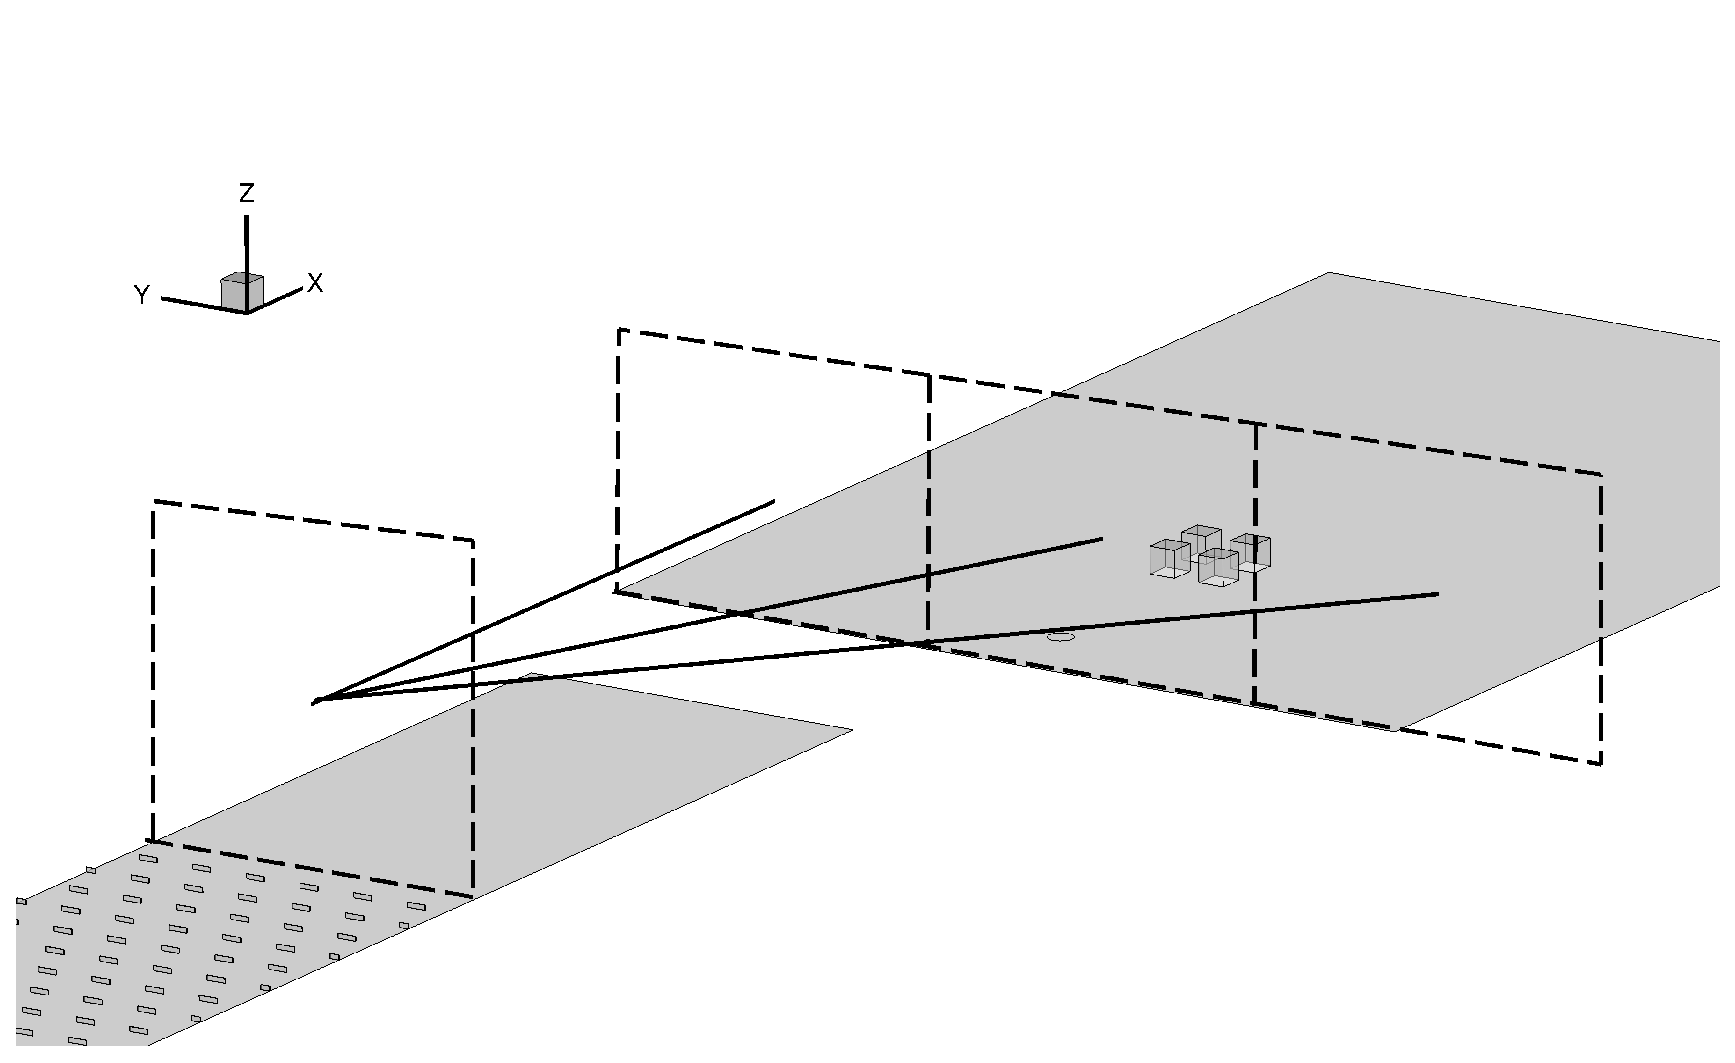
\includegraphics[width=0.9\textwidth]{figures/b8inst.eps}
	\caption{The instantaneous velocity field from the previous simulations is inserted 
	as the inflow boundary condition. The small shaded strips represent roughness elements 
used for creating the boundary layer.}
\label{fig:inlet}
\end{figure}
%
\subsection{Implementation in Fluent}\label{Fluent}
 The configurations used are 
briefly stated in the list below. The boldfaced objects are the default settings which will be 
compared with optional settings.
\begin{enumerate}
		\item Models
			\begin{itemize}
					\item Viscous -- LES with Smagorinsky SGS model
					\item Species Transport using a volume weighted mixing law
				\end{itemize}
		\item Materials
			\begin{itemize}
					\item	Defining air and the gas to be released
				\end{itemize}
		\item Boundary conditions
			\begin{itemize}
					\item Main inflow:  Read from files using several UDFs
					\item Gas source:  Specified mass flow rate $50l/\min$
					\item Floor and cubes:  No slip conditions
					\item Walls and ``sky''Free slip conditions by specifying symmetric stress
				\end{itemize}
		\item Solution Methods
			\begin{itemize}
				\item Pressure-Velocity Coupling Scheme:  SIMPLE
				\item Gradient:  Least Squares Cell Based
				\item Pressure:  Second Order
			\textbf{\item Momentum:  Bounded Central Differencing}
			\textbf{\item Air:  Second Order Upwind}
			\textbf{\item Transient Formulation:  Bounded Second Order Implicit }
				\end{itemize}
\label{tab:Fluent}
	\end{enumerate}
In addition to these standard settings various user defined 
functions (UDFs) had to be implemented in order to define the input velocity. 
The solution methods stated in the list above are the default settings for a problem of this type. 
The discretization for both the momentum equation and the time-development are bounded, which
implies the use of some extra parameters to stabilize the solution. 
A second order implicit discretization in time is given as 
\begin{align}
	\frac{\partial\phi}{\partial t}= \frac{3\phi_n-4\phi_{n-1}+\phi_{n-2}}{2\Delta t}.
	\label{eq:u2o}
\end{align}
This discretization provides an error term of order $O(\Delta t^2)$. The bounded second order implicit scheme 
provides a similar discretization with the bounding factors
$\beta_{n+1/2}$ and $\beta_{n-1/2}$. How these variables are chosen is not stated explicitly in the 
Fluent Theory Guide~\cite{theoryguide}, but the scheme is given as
\begin{align}
	\frac{\partial\phi}{\partial t}= \frac{(1+\beta_{n+1/2})\phi_n
	-(1+\beta_{n+1/2}+\beta_{n-1/2})\phi_{n-1}+\beta_{n-1/2}\phi_{n-2}}{\Delta t}.
	\label{eq:u2ob}
\end{align}
Unless the bounding factors are chosen such that they correspond to the discretization in~\cref{eq:u2o}
the error term will be of order $O(\Delta t)$. 
The second order upwind method used for the discretization of the species is a method which 
adds a diffusion term of order $O(\Delta t)$ and does in this way stabilize the numerical 
method by reducing the order of accuracy. 

By choosing different solution methods one can expect to obtain slightly different run times
and solutions. Based on the assumption that Fluent provides stable, diffusive solutions
the momentum, air and transport schemes from point 4 in the list above will be exchanged
for less diffusive schemes.


\subsection{Reading the inflow}
The inflow at each timestep is specified componentwise in separate files.
For each timestep the file corresponding to the current flow time is read
and interpolated to the nodes defining the inflow in Fluent. 
It is necessary to take advantage of the built-in \verb|DEFINE| macros Fluent has available,
more information about these can be found in the \emph{Fluent UDF manual}~\cite{UDF}.
The whole process is divided into the following three steps:
			\begin{enumerate}
				\item \verb|DEFINE_INIT(name,*d)| - Defining the interpolation
					algorithm. Only executed when the flow is initialized.
				\item \verb|DEFINE_ADJUST(name,*d)| - Reading the inflow for the current 
					timestep and defining the components of the inflow. Executed at 
					the beginning of each timestep.
				\item \verb|DEFINE_PROFILE(name,*t,i)| - Applying the predefined
					interpolation	algorithm and imposing the interpolated values 
					to each node in the inflow. 
				\end{enumerate}

In order to clarify the approach the general pseudo code is listed below.
\begingroup
\fontsize{10pt}{12pt}
\begin{alltt}
	/* Pseudo code */ 
define interpolation algorithm  (``DEFINE_INIT'')
\textbf{\textbf{for}} each timestep \emph{T}
  Read inflow (``DEFINE_ADJUST'')
  \textbf{for} each node \emph{N} and velocity component \emph{V} on inflow boundary 
    \emph{V}(\emph{N}) = doInterpolation(N) (``DEFINE_PROFILE'')
  \textbf{endfor}
  solve
\textbf{endfor}
\end{alltt}
\endgroup

%\begin{alltt}
	%/* Fluent pseudo code */
	%DEFINE_INIT(initialize,domain)
	%for timestep \emph{T}
    %DEFINE_ADJUST(read_components,domain)
    %while( continuity residual > \emph{tol})
      %DEFINE_PROFILE(xVel,thread,i)
      %DEFINE_PROFILE(yVel,thread,i)
      %DEFINE_PROFILE(zVel,thread,i)
%\end{alltt}

In order to make the interpolation algorithm run efficiently some global variables are stored. 
These variables will be deleted after a Fluent session and it is necessary 
to redefine them for every new Fluent session. Note that \verb|DEFINE_INIT| is only executable
at the initialization of the flow. There is therefore necessary to initialize the global 
variables in a different way. This is solved by creating the 
UDF \verb|DEFINE_ON_DEMAND| which can be executed at any given point and thus 
initialize the global variables when starting up Fluent in the middle of a 
simulation.
		
The interpolation algorithm used for this experiment is an inverse distance
interpolation using the four closest points and the inversed distance
squared as weights. 

\subsection{Cases investigated}
One of the main objectives of this work is to investigate the Fluent solver and 
how it manages to simulate gas dispersion. In order to get a good understanding of 
how the solver works and how the different settings in Fluent affect the solution,
several comparison studies were performed. The results are presented in chapter~\ref{results}, 
but for clarity the different cases investigated will be stated and motivated here. 

\begin{enumerate}
    \item \textbf{Fluent/CDP/Wind tunnel experiment}\\
        comparing the solution to the data from CDP simulations and wind tunnel experiments
    \item \textbf{Variation in solver settings}\\
        Fluent automatically suggests certain solver settings depending on the 
        problem to be solved. To find out if it was possible to make the solver more 
        efficient and accurate, it was experimented with several of the schemes available.
    \item \textbf{The effect of the SGS model}\\
        Comparing solutions with and without an SGS model. In the central parts of the domain
        the mesh is very fine, $\Delta \sim \eta$, where $\eta$ is the Smagorinsky length scale 
        which is estimated to be approximately $1.5$mm in section ~\ref{sgs}. 
        Most of the turbulent structures are resolved and the SGS model should be less important. 
    \item \textbf{Variation in gridsize}\\
        In order to find out how good the resolution of the mesh needs to be,
        solutions using $N=6.200.000 ,N/2\text{ and } N/4$ nodes is compared. For the coarser meshes 
        the SGS model will be more important, and a lot of computational time can be saved 
        if the SGS model is found to provide good results. This is also an important test
        to check that grid convergence is obtained.
    \item \textbf{Fluent/CDP/Wind tunnel experiment - Heavy gas}\\
        Comparing the solution to the data from CDP simulations and wind tunnel 
        experiments for heavy gas release. The same volume of gas is inserted to the domain, 
        and the settings of the solver is as similar as possible to the default case for 
        neutral gas. The only changes necessary in Fluent was switching on gravity and adding
        CO$_2$ as a species. 
\end{enumerate}

\section{Results and discussion}\label{results}
This section contains the results from the simulations compared with
the experimental wind tunnel measurements and the simulations performed with CDP\@.
In order to generate the results the values in table~\ref{tab:output} are being 
written to file from Fluent. 
	
\begin{table}[h]
    \begin{center}
        \begin{tabular}[b]{l|c}
            $x_i$ 	 & Coordinates  					\\\hline
            $u_iu_i$ & Turbulent normal stresses		\\\hline
            $u_1u_3$ & Reynold's stress component		\\\hline
            $U_i$    & Velocity components				\\\hline
            $C$      & Concentration of released gas	\\\hline
            $c$      & Fluctuating part of the concentration
            \end{tabular} 
        \caption{Output variables from simulations performed with Fluent.}
\label{tab:output}
    \end{center}
\end{table}

All values are either predefined in Fluent or easily calculated from 
the available values. All values are averaged in time, with a sample time specified in each case. 
All time-averaged variables will be denoted $\overline{var}$, and the variables 
averaged in both time and space will be denoted $\langle var \rangle$.

\subsection{Boundary layer creation}
Before any gas can be released the profile of the flow and the boundary layer 
have to be correctly estimated.
The Reynold's stresses and the scaled velocity variable is therefore compared 
with the wind tunnel experiment. 
The results in figure~\ref{fig:bl} show good agreement with the experimental data
apart from an underestimation of the first normal stress.
The sharp peaks right above ground level are due to the roughness elements
(see figure~\ref{fig:inlet}) used to create the boundary layer.
One can clearly see from $\langle uu\rangle$ how this stabilizes 
inside the domain where no roughness elements are present.
%
\begin{figure}[h]
  \centering
  \begin{subfigure}[b]{0.40\textwidth}
	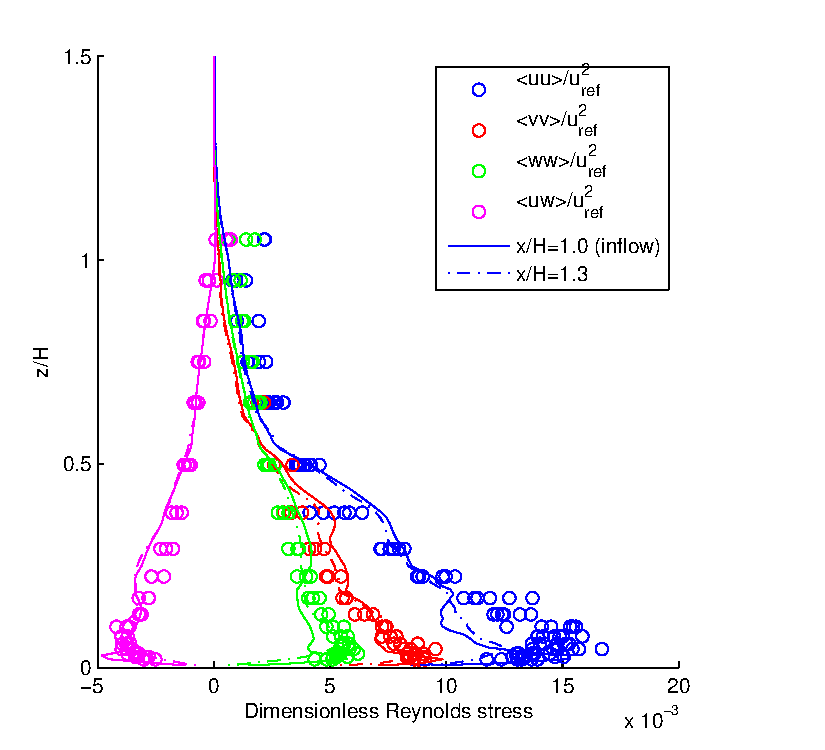
\includegraphics[width=\textwidth]{figures/rey.pdf}
  \end{subfigure}%
  \quad
  \begin{subfigure}[b]{0.40\textwidth}
	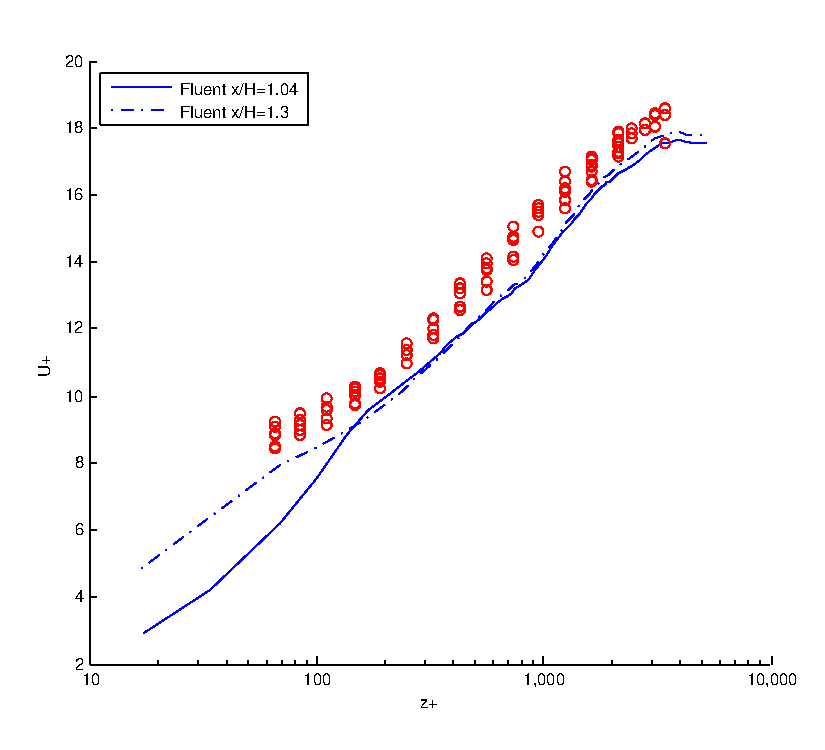
\includegraphics[width=\textwidth]{figures/uplus2.pdf}
  \end{subfigure}
          %(or a blank line to force the subfigure onto a new line)
  \vspace{-0.1\baselineskip}
  \caption{Lateral ($-1\leq y/H \leq 1$) and time-averaged wind field at the inflow 
and at $x/H = 1.3$, compared with experimental data. (a) Non-dimensional Reynold's stress 
plotted against $z/H$. (b) $U^+$ plotted against $z^+$}
\label{fig:bl}
\end{figure}
%

The reduction of stress is also visible in~\ref{fig:bl}(b). $U^+ = U_{ref}/U^*$ increases 
slightly in the buffer region $(5<z^+<200)$ implying a reduction in the friction velocity 
estimated by the relation $U^* = \sqrt{-\langle uw\rangle}$. The averaging of $uw$ in this particular
estimation of $U^*$ is done in time and within the spatial domain $-1\leq y/H \leq 1$ 
and $0\leq z/H \leq 0.2$. 
\newpage
\subsection{Neutrally buoyant gas}
%
\begin{figure}[h]
  \centering
  \begin{subfigure}[b]{0.48\textwidth}
	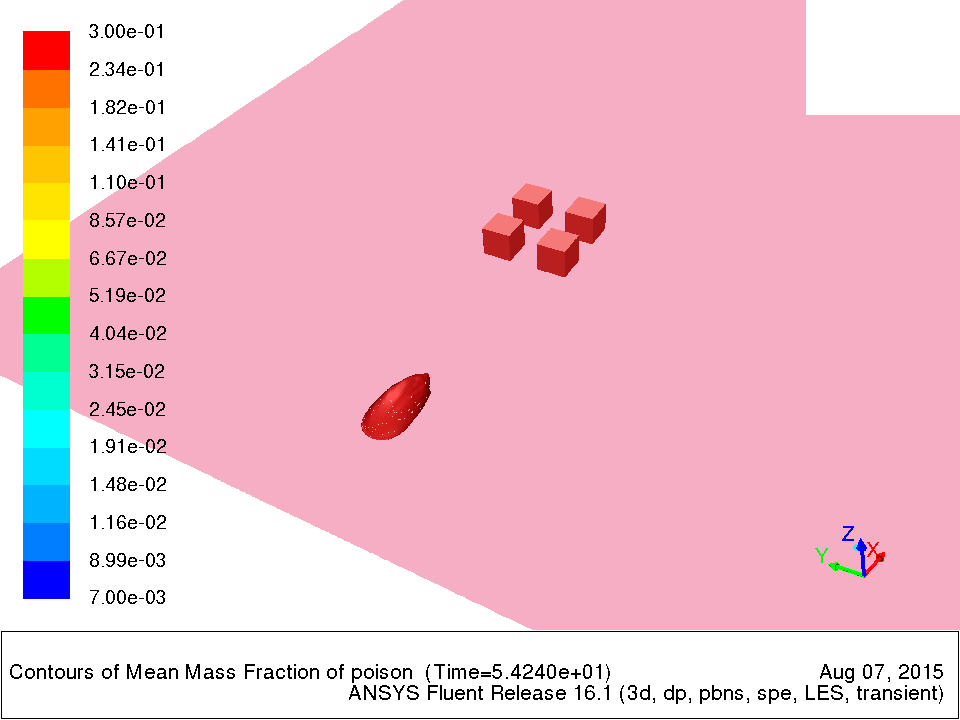
\includegraphics[width=\textwidth]{figures/iso3-def.png}
  \end{subfigure}%
  \quad
  \begin{subfigure}[b]{0.48\textwidth}
	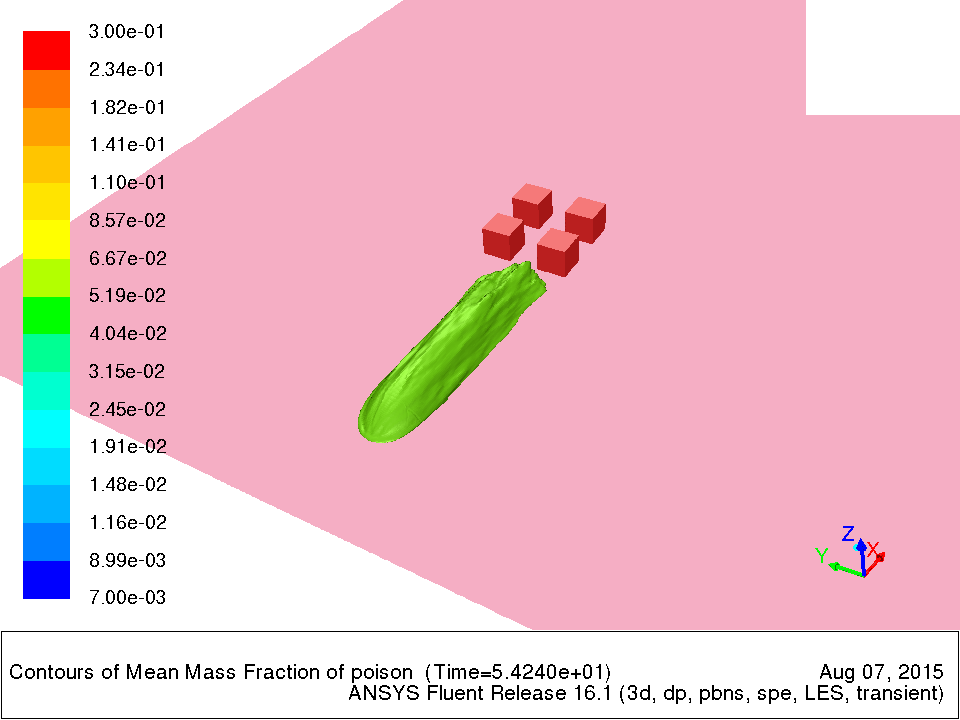
\includegraphics[width=\textwidth]{figures/iso06-def.png}
  \end{subfigure}
  \begin{subfigure}[b]{0.48\textwidth}
	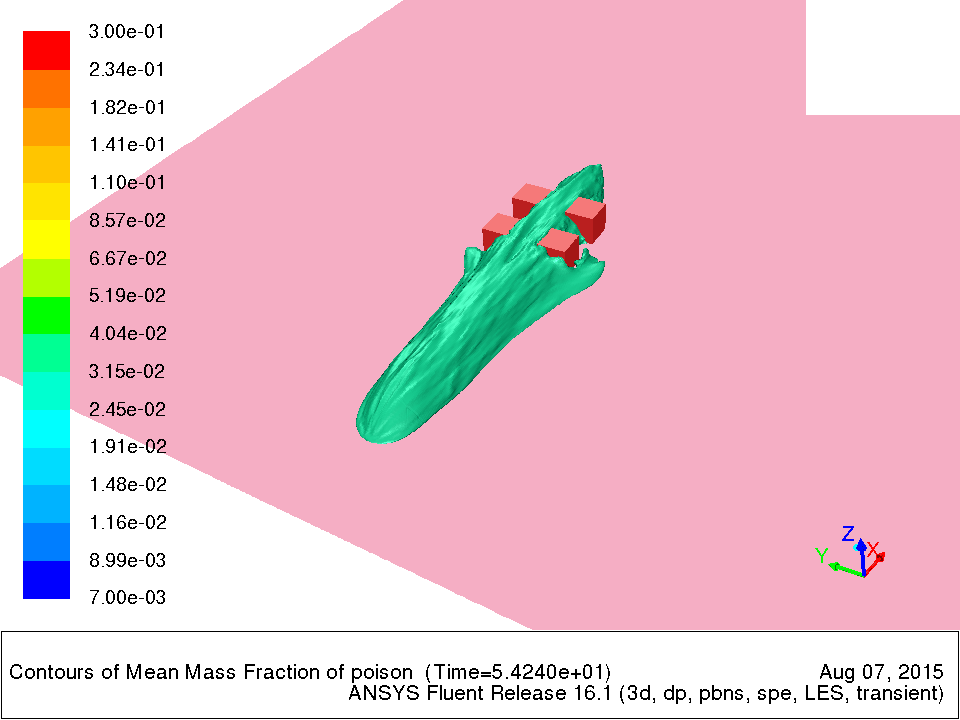
\includegraphics[width=\textwidth]{figures/iso03-def.png}
  \end{subfigure}%
  \quad
  \begin{subfigure}[b]{0.48\textwidth}
	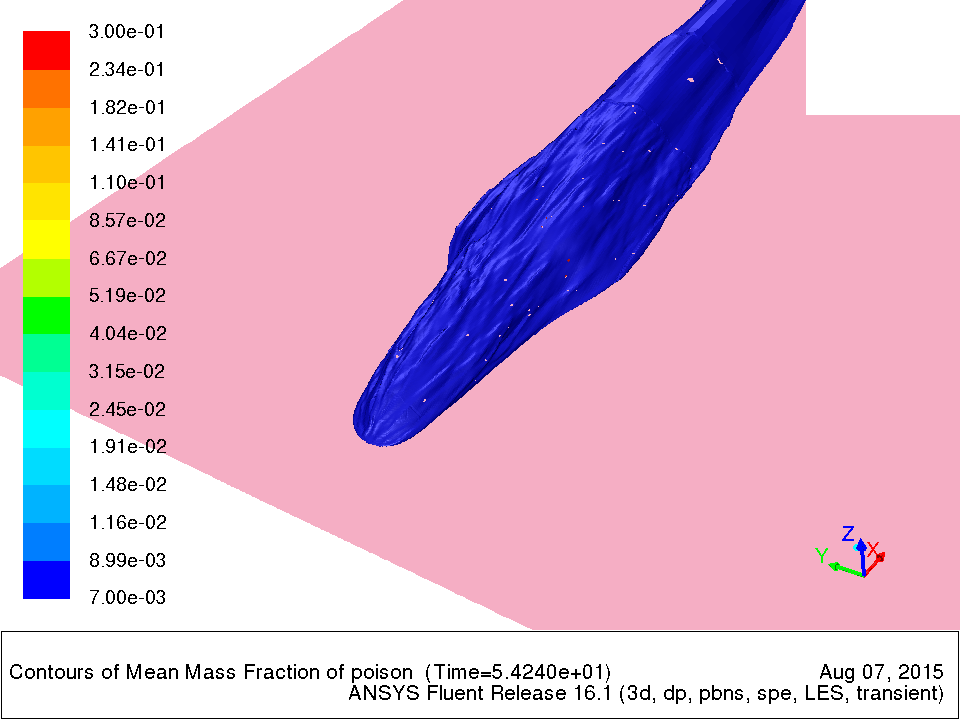
\includegraphics[width=\textwidth]{figures/iso007-def.png}
  \end{subfigure}
          %(or a blank line to force the subfigure onto a new line)
  \vspace{-0.1\baselineskip}
\caption{Species concentration plotted on iso-surfaces of time-averaged
	mass fraction for neutral release. The sample time is $11.04$ seconds.
	(a) C = 0.3, (b) C = 0.06, (c) C = 0.03, (d) C = 0.007. }
\label{fig:iso}
\end{figure}
%
In figure~\ref{fig:iso} the mass fraction of the released gas is fixed on the surfaces. 
The results show a very smooth surface for the different values for the concentration.
The plume is slightly shifted towards negative y-direction, this indicates that the sampling time
should be even longer. 

Figure~\ref{fig:cH} shows the scaled concentration along the dashed 
lines in figure~\ref{fig:layout}. The experimental data and Fluent provide a plume that is 
slightly shifted towards negative $y$, whereas CDP has a shift towards positive $y$.
The shift in the experimental data could be explained by 
some geometrical asymmetry or insufficient time used for measuring. The simulated results are 
probably not symmetric because the sampling time is not sufficiently long, and since the 
simulations are invoked at different times the asymmetry is different. Another explanation
could be that in Fluent the inflow condition is translated so that it corresponds to a 
symmetric distribution of roughness elements in the creation of the boundary layer. 
The simulated width of the plume is consistent with the experimental data, 
and the maximal concentration is also very similar, but somewhat higher 
for the measurements downstream in the experimental data. 
%
\begin{figure}[!h]
	\centering
	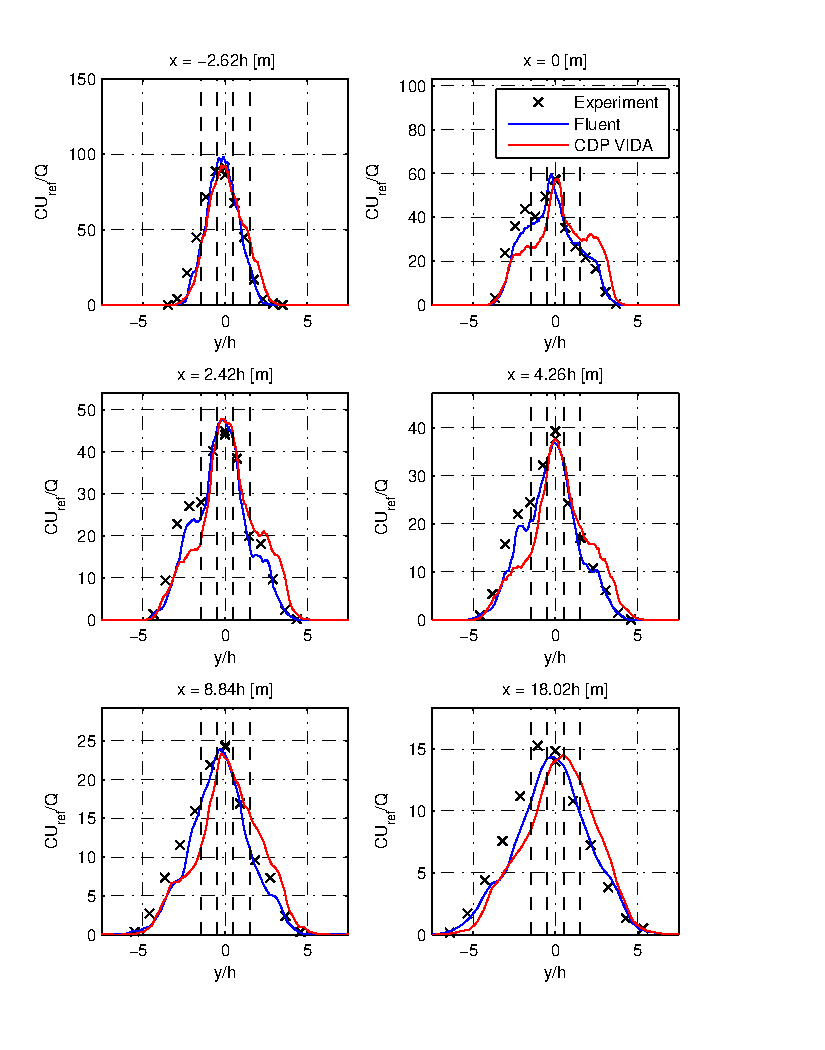
\includegraphics[width=0.8\textwidth]{figures/cH.pdf}
	\caption{Time-averaged concentration with a sample time of $12.48$ s at $z/H = 0.025$ plotted horizontally and scaled 
	with the free-stream velocity and emission rate. Compared against wind tunnel data.
Two dashed lines on either side of the centerline represent the canyon.}
\label{fig:cH}
\end{figure}
%

%and the height is also very similar apart from the first 
%line where we see an overshoot in the center of the simulated results. 

\clearpage
%
\begin{figure}[!h]
	\centering
	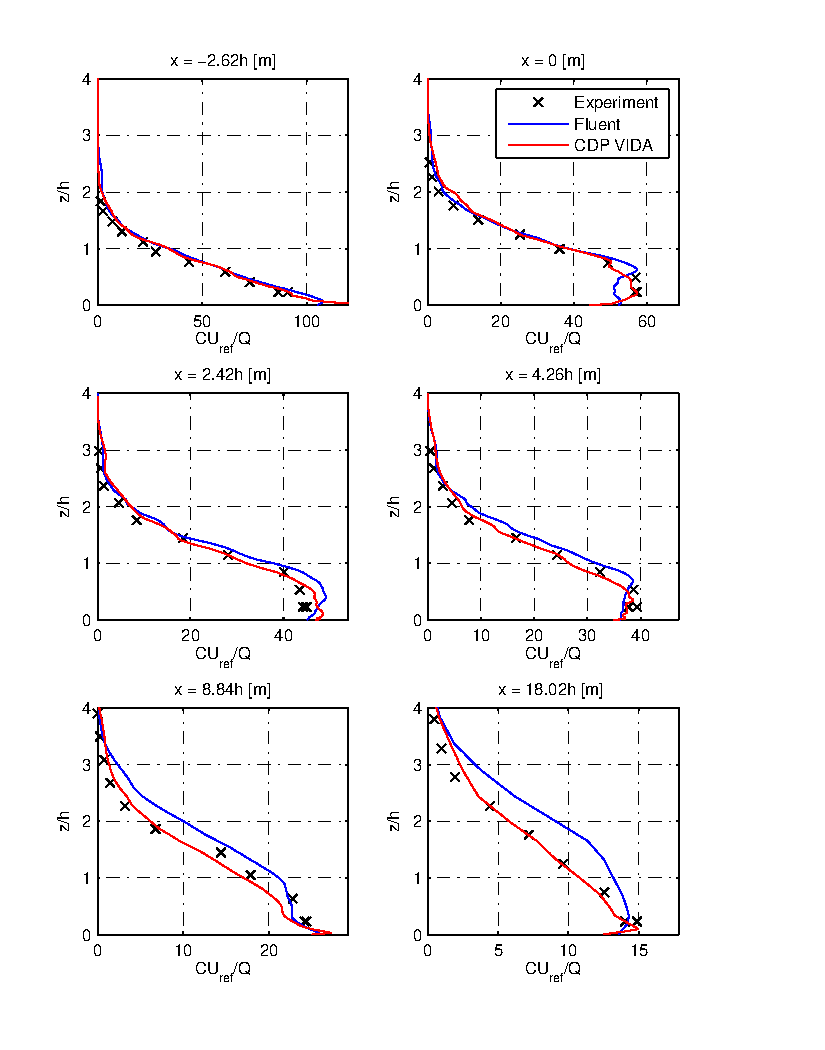
\includegraphics[width=0.8\textwidth]{figures/cV.pdf}
	\caption{Time-averaged concentration with a sample time of $12.48$ s at $y/H = 0$ plotted vertically and scaled with the
		free-stream	velocity and emission rate. Compared against wind tunnel data.}
\label{fig:cV}
\end{figure}
%

The computational results in figure~\ref{fig:cV} capture very well the 
structure of the concentration in the plane $y=0$. Further downstream the differences 
increase, and Fluent has a tendency to overestimate the concentration. 
Close to the wall the solutions are not identical, but all the data estimates roughly the 
same peak concentration. 
%Both the height and the development of the plume is predicted very well with the simulations. 

\newpage
%
\begin{figure}[!h]
	\centering
	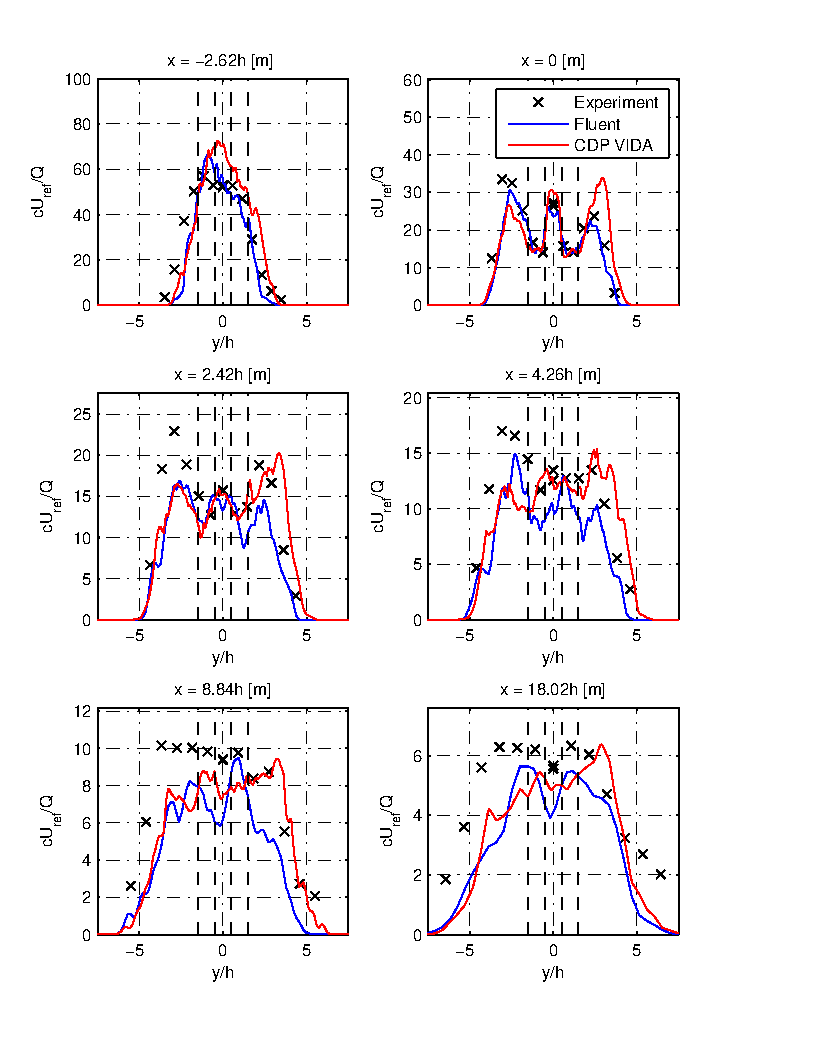
\includegraphics[width=0.8\textwidth]{figures/cfluctH.pdf}
	\caption{Fluctuating concentration with a sample time of $12.48$ s at $z/H = 0.025$ plotted horizontally and
	scaled with the free stream velocity and emission rate. Compared against wind tunnel data.} 
\label{fig:cfluctH}
\end{figure}
%
The fluctuation of the released gas concentration is plotted against the wind tunnel data in figure~\ref{fig:cfluctH}.
Also in this plot the simulated and experimental data give similar results. 
One can clearly see how the simulation captures the structures of the fluctuation. 
%
\subsection{Performance testing - (removed/do again due to cluster instabilities?)}
A small performance test was performed to evaluate Fluents ability to run on multiple cores.
\begin{table}[h]
	\centering
	\begin{tabular}{|c|c|c|c|}
		\hline
		Cores & Time (h)& Speedup per iteration  & Total speedup \\		\hline
		40		& 94,7& 1				 & 1						 \\
		80		& 51,6& 1,9			 & 1,8					 \\
		120		& 25,8& 2,9			 & 3,7					 \\	\hline
	\end{tabular}
	\caption{Small performance test on 4000 iterations.}
	\label{tab:perfscaling}
\end{table}
In table~\ref{tab:perfscaling} the simulations are not executed on the same interval in time, but the 
flow and gas-release is well-developed in all 3 cases.
This can affect the convergence-rate and thus also the total run-time.
The data does however indicate a good speedup for a number of cores in this range. 
For $120$ cores the convergence went drastically faster than for the two others, this is what
cause the surprisingly good total speedup. A possible explanation could be that the 
local preconditioner used in the calculation results in a
faster convergence when the problem is decomposed to 120 cores. 
%
\subsection{Testing of discretization schemes in Fluent}\label{chap:perf}
As mentioned in Section~\ref{Fluent}, several of the solution methods have been tested and a small 
performance-test is done. The discretizations referred to as default are the ones stated in boldface
in the list in Section~\ref{Fluent}. The performance data are all relative to the all-default 
	solution given explicitly in the last row. Relative convergence refers to the number of times convergence is reached relative to the all-default
case.
\begin{table}[!h]
	\centering
	\begin{tabular}{|l|c|c|c|c|c|c|c}
		\hline
			& \multicolumn{3}{|c|}{Discretization} & \multicolumn{3}{|c|}{Relative performance}\\ \hline
		Settings & Time& Momentum& Species														 & Time per it &Convergence&	 Total time  \\ \hline
			1	& 2nd				&Default 				&Default										 & 0.92				&	1.2				 & 0.90					\\ 
			2	& Default   &3rd MUSCL		  &Default										 & 0.99				&	1.4				 & 0.83					\\ 
			3	& Default   &Default 				&3rd MUSCL									 & 1.01				&	1.2				 & 0.99					\\ 
			4	& 2nd				&3rd MUSCL		  &3rd MUSCL									 & 0.93				&	1.4				 & 0.80					\\ \hline \hline
			Default				& 2nd bounded		& bounded CD		 & 2nd upwind& 1.85 sec		&	69\%	     & 94.7 hours			\\ 
			\hline
	\end{tabular}
	\caption{Performance test on 4000 timesteps, or 6.4 seconds for different solution method settings in Fluent,
		all with convergence criteria $5\cdot10^{-8}$ on the residual from the continuity equation, and a maximum of 50 iterations per timestep.
		The simulations are all performed on 40 cores. Convergence is here defined as the number of 
		timesteps which reached convergence divided by the total number of timesteps. }
\label{tab:performance}
\end{table}
%
\newpage
%
\begin{figure}[h]
	\centering
	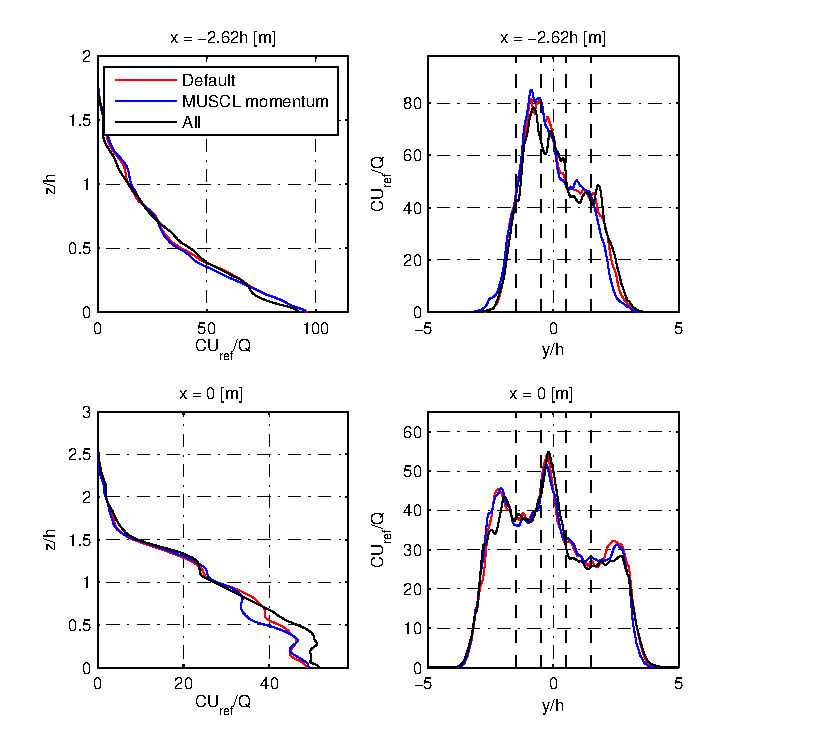
\includegraphics[width=0.8\textwidth]{figures/perftest.pdf}
	\caption{Time-averaged concentration with $5.92$ s of sampling at $z/H = 0.025$ plotted horizontally and scaled 
	with the free-stream velocity and emission rate.}
\label{fig:default-not}
\end{figure}
%
The performance results presented in table~\ref{tab:performance} reveal that the performance 
is not affected in any significant way by the scheme chosen for the species. 
This is as expected since the simulation 
is done with a neutrally buoyant gas which will have very little impact on the flow.
By changing the time discretization the convergence rate increases slightly, 
while the calculation time drops by almost 10 \%. 
With the 3rd order MUSCL scheme for momentum, convergence is increased by 70 \%, and with a 
small change in the computational time at iteration level the total runtime is decreased by 17 \%.
The data in table~\ref{tab:performance} will depend on the convergence criteria and the maximum 
number of iterations allowed, but it gives an indication of how the different solver settings compare.  
%
%
%\begin{figure}[h]
	%\centering
	%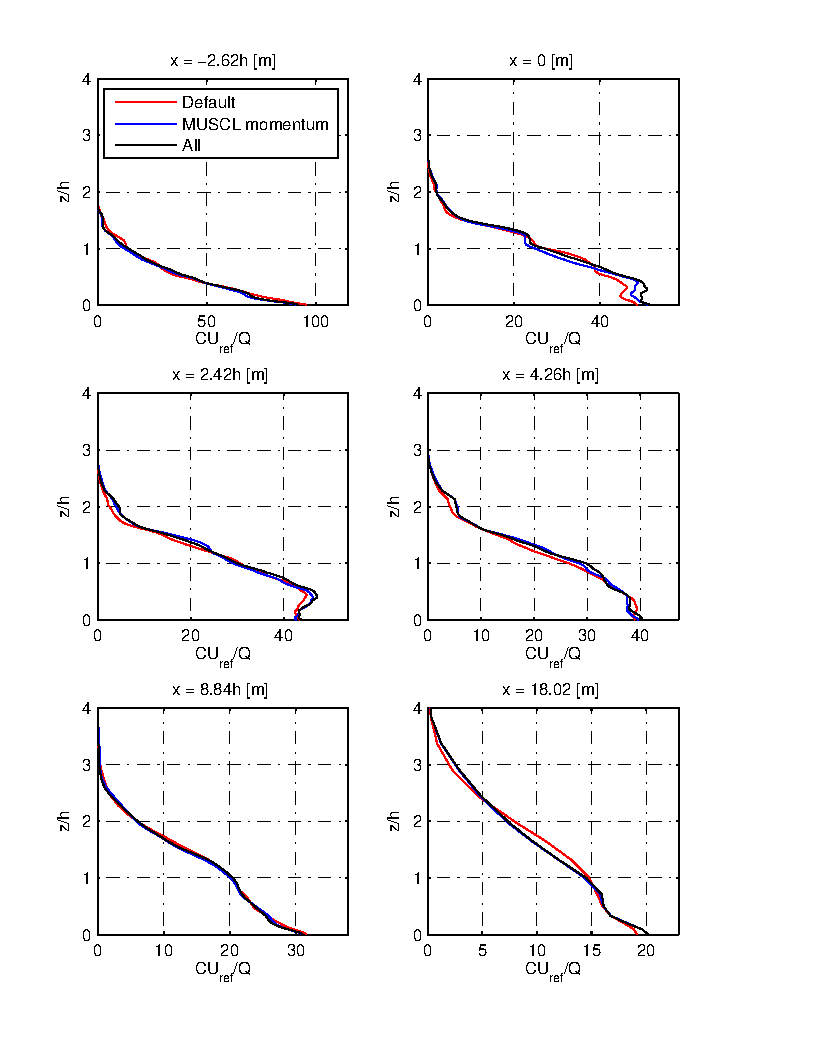
\includegraphics[width=0.8\textwidth]{figures/cVcompcases.pdf}
	%\caption{Time-averaged concentration with $5.92$ s of sampling at $y/H = 0$ plotted vertically and scaled with the
		%free-stream	velocity and emission rate.}
	%\label{fig:cVcompcases}
%\end{figure}
%
The change which has the most significant impact is the momentum discretization, 
in figure~\ref{fig:default-not} %and~\ref{fig:cVcompcases} 
the results after $5.92$
seconds is presented. The shape of the plume is very similar in all cases, the width is 
identical and the height is also very similar. There are however small deviations that could
potentially make the plumes even more distinct over time, in order to better understand the effect 
of the schemes the simulation was done over a larger time-interval.
\newpage
Since discretization settings 
nr. 4 in table~\ref{tab:performance} (from now on referred to as the tuned case) 
performed best this was a natural choice for a longer comparison against the default case. 
The results are presented in figure~\ref{fig:perftest}.
After a longer sampling time the effects of the default bounded schemes recommended by Fluent 
become clearer. Although the results have similarities with respect to the shape of the plume 
the tuned case consistently underestimates the concentration.
%
%\newpage
%
\begin{figure}[h]
	\centering
	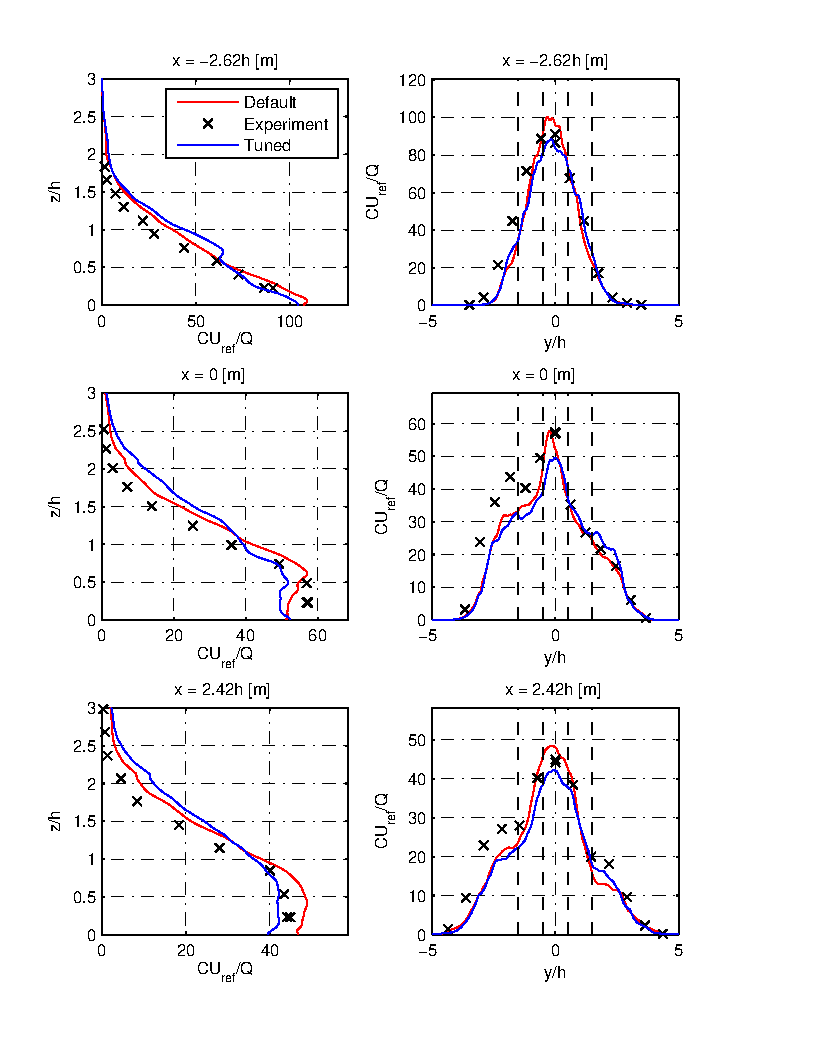
\includegraphics[width=0.8\textwidth]{figures/default-not.pdf}
	\caption{Time-averaged concentration with $12.48$ s of sampling at 
        $y = 0$ to the left and $z/H = 0.025$ to the right. Both plots are scaled 
	with the free-stream velocity and the emission rate.}
\label{fig:perftest}
\end{figure}

%
%An interesting difference is in 
%the last plot in figure~\ref{fig:cVcompcases}, where the default scheme predicts a higher
%concentration for $ 1 \leq z \leq 2$. 
%The fact that the data from the wind tunnel experiment and from CDP also predicts 
%a lower concentration than Fluent (figure~\ref{fig:cV}) in this domain gives reason to believe that 
%by changing the discretization schemes one might be able to provide better estimates for
%the species concentration.
%%
\subsection{The effect of the subgrid-scale model} \label{sgs}
Performing an LES implies resolving the larger turbulent structures and modelling the smaller ones using
an SGS model. In this case the modelling is done using the Smagorinsky-Lilly SGS model.
By using a sufficiently fine grid, the effect of the unresolved structures will have very 
little influence on the rest of the flow. The viscous length scale is the scale that is 
appropriate to use in order to resolve all structures. An estimation of this scale is given as 
\begin{align}
    \delta_v=\sqrt{\frac{\nu}{\mathcal{S}}}\approx 1.5\text{mm}
	\label{eq:lengthscale}
\end{align}
$\nu$ is here the efficient kinematic viscosity and $\mathcal{S}=|S_{ij}|$ is the magnitude of 
the strain-rate tensor. The estimated value is calculated along the dotted measurement lines
in figure~\ref{fig:layout}.

The grid size $\Delta = V_{cell}^{1/3}$, which in this case is the same as the filter size 
used in this work, is of the same order as $\delta_v$.
The fact that $\Delta \sim \delta_v$ means that the SGS model might not be as important since 
most of the energy spectrum is resolved. A comparison was done between dynamic Smagorinsky
and no SGS model, the results are plotted in figure~\ref{fig:cHcompSGS}. % and~\ref{fig:cVcompSGS}. 
The plots clearly show that even without the SGS model Fluent is able to capture the shape of the 
plume. It is worth to mention that the
sampling time is not sufficiently long for the plume to be stabilized, so it is hard to determine 
whether the simulation without an SGS model will be able to predict a plume that is similar to the 
measured data from the wind tunnel experiment. But the effect of the SGS model is indisputable,
especially the horizontal plots illustrates how it reduces the asymmetry of the plume.  

By comparing the performance as done to the tests in table~\ref{tab:performance} one finds that 
by omitting the SGS model the computational time per iteration decreases with less than 5\% and 
that convergence is about 10\% slower. The resulting effect is that the total computational time 
does not change.

\newpage
%
\begin{figure}[h]
	\centering
	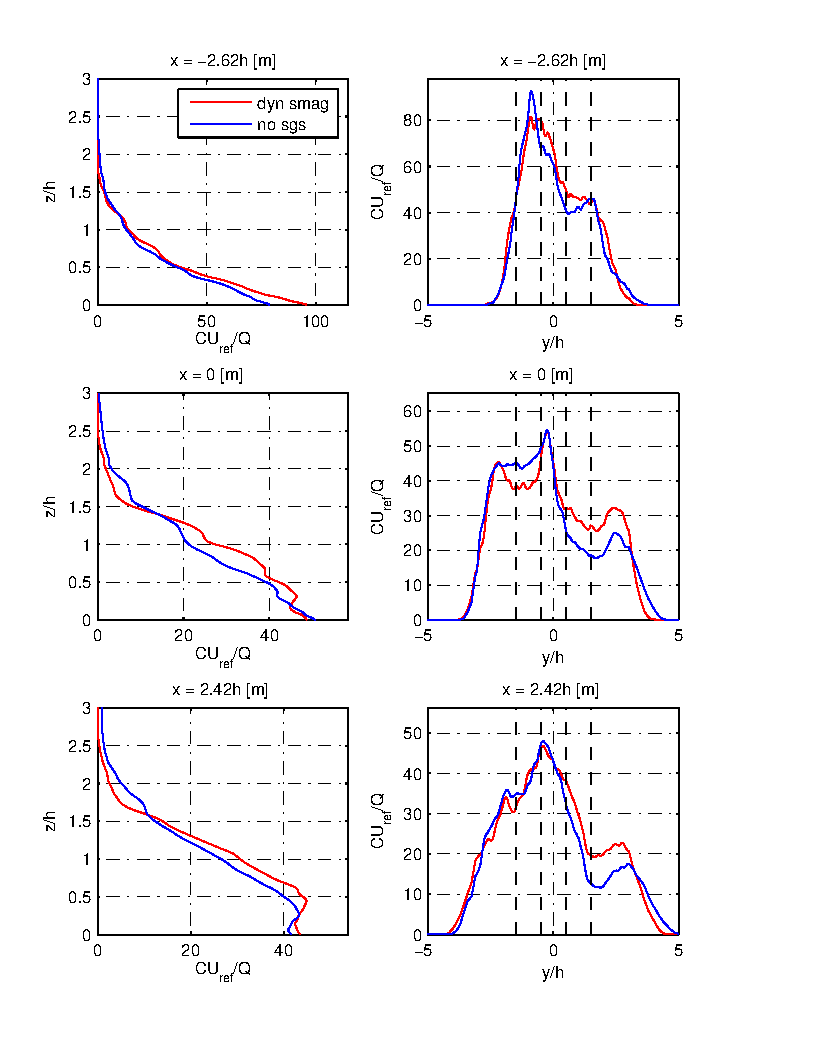
\includegraphics[width=0.8\textwidth]{figures/sgsmodel.pdf}
	\caption{Dynamic Smagorinsky compared with no SGS model. Time-averaged concentration with $5.92$ s of sampling at $z/H = 0.025$ plotted horizontally and scaled 
	with the free-stream velocity and emission rate.}
\label{fig:cHcompSGS}
\end{figure}
%
\newpage
%
\subsection{Grid size}
By reducing the number of grid cells, the result should yield a less
accurate solution. In figure~\ref{fig:ref-coarse} three distinct meshes
are compared. 
The difference between the solutions are not critical, they all estimate a plume similar 
to the experimental one.
With coarser mesh Fluent does however consistently estimate a lower peak, something that 
would suggest a poorer approximation of the conserving laws of passive scalars.
%
\begin{figure}[h]
    \centering
    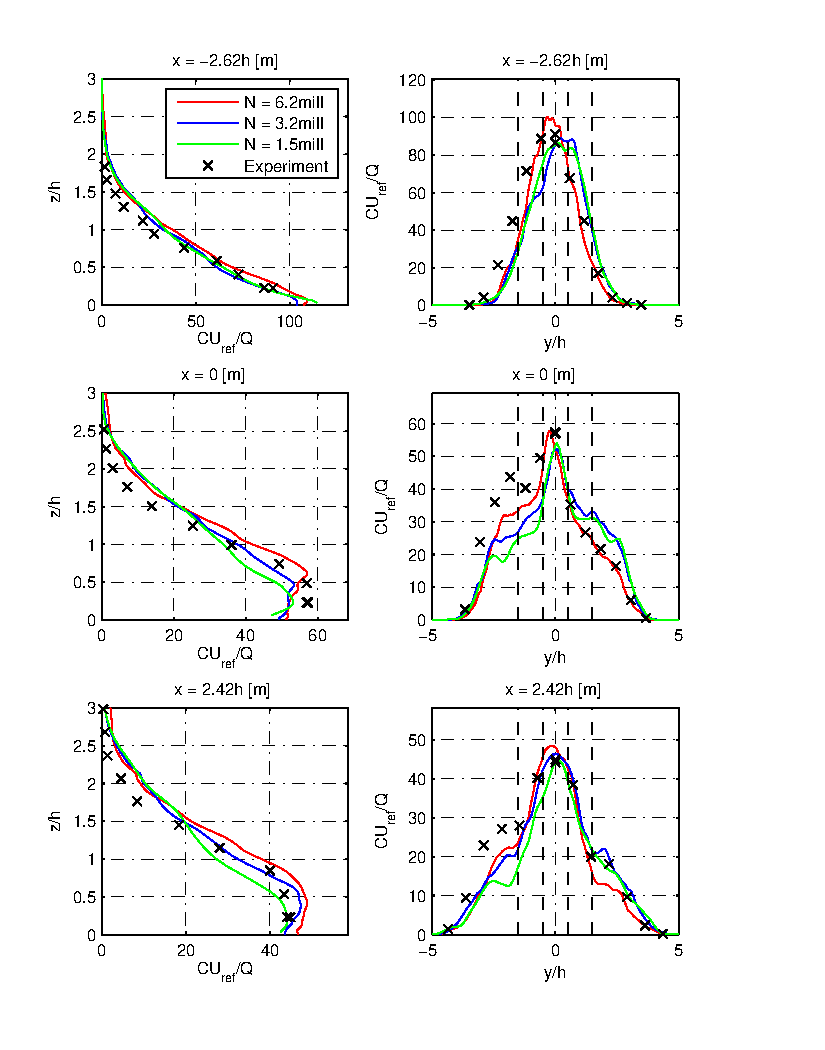
\includegraphics[width=0.8\textwidth]{figures/ref-coarse.pdf}
    \caption{Time-averaged concentration with $12.48$ s of sampling at $y/H = 0$ to the left 
        and $z/H=0.025$ to the right. All concentrations are scaled with the
        free-stream	velocity and the emission rate.}
\label{fig:ref-coarse}
\end{figure}
%
The semi-coarse mesh is created by lowering the resolution along the edges, but the resolution-levels
are maintained. More specifically $\Delta x$ and $\Delta y$ from table~\ref{tab:gridsize}
is multiplied by a factor of $1.4$ while $\Delta z$ remains unchanged.
The coarsest mesh is identical to the semi-coarse mesh but without the finest
refinement layer, in other words $R1 = R2$.

%\begin{figure}[h]
	%\centering
	%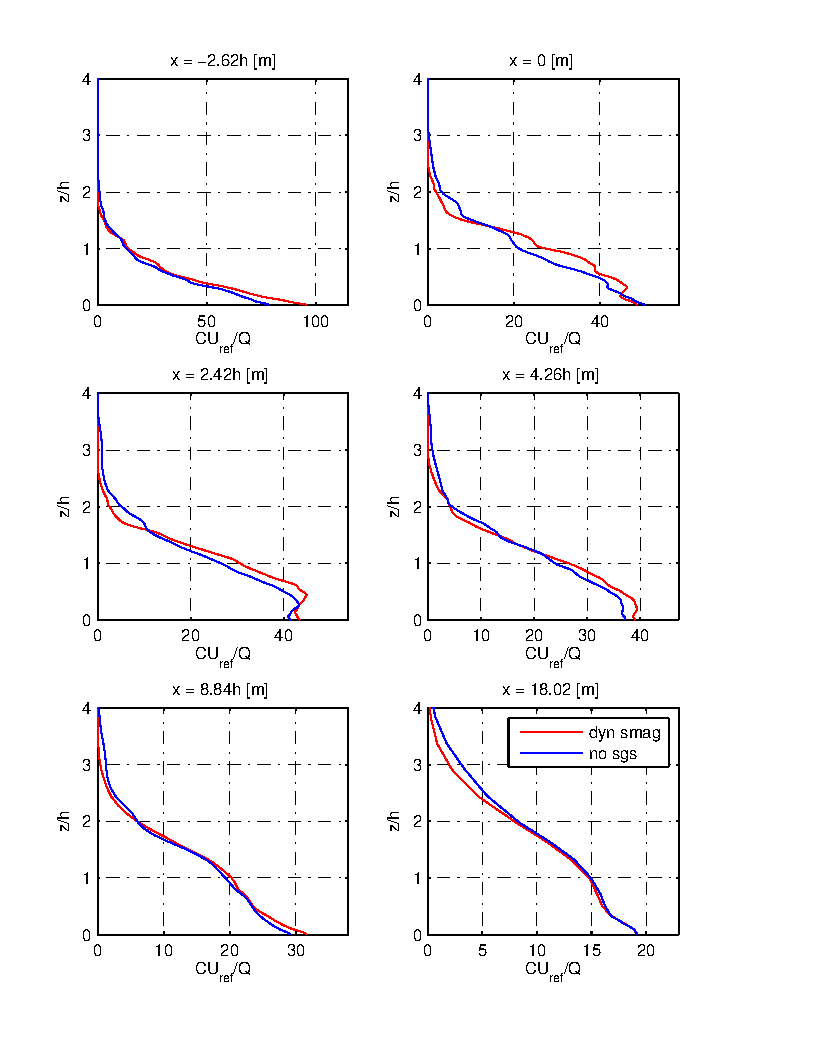
\includegraphics[width=0.8\textwidth]{figures/cVcompsgs.pdf}
	%\caption{Dynamic Smagorinsky compared with no SGS model. Time-averaged concentration with $5.92$ s of sampling at $y/H = 0$ plotted vertically and scaled with the
		%free-stream	velocity and emission rate.}
	%\label{fig:cVcompSGS}
%\end{figure}
%
%\subsection{The effect of the discretization schemes}
%In chapter~\ref{chap:perf} it was experimented with different discretization schemes and the 
%performance was significantly improved from the default settings recommended by Fluent.
%Although the performance test suggest a change of settings the correctness of the new scheme 
%is even more important. The changes suggested by the fastest scheme 
%(simulation 4 in table~\ref{tab:performance}) was done and the simulation 
%was performed for 12.48 seconds. Changing the time-descretization from \textit{bounded 2nd order} to 
%\textit{2nd order} suggests a more correct and less smooth solution. The Fluent manual also describes 
%the \textit{3rd order MUSCL}-scheme as a more agressive option to \textit{Bounded CD}. Put in a 
%simpler way, one can expect a more correct solution if it turns out to be sufficiently stable.
\section{Heavy gas}
A passive scalar does not have any effect on the velocity field so the computational 
challenges are similar to the ones encountered when simulating a common flow problem. 
When a heavy gas is released into a flow it has to be treated as an active scalar and 
it will affect the initial velocity field. This is a computationally more demanding problem, 
but nevertheless a realistic case and it is important to verify that our computational software 
is able to provide good estimates. The measurments are done in the same fashion as for neutral 
gas, but at slightly different positions downstream.
%
\begin{figure}[!h]
    \centering
    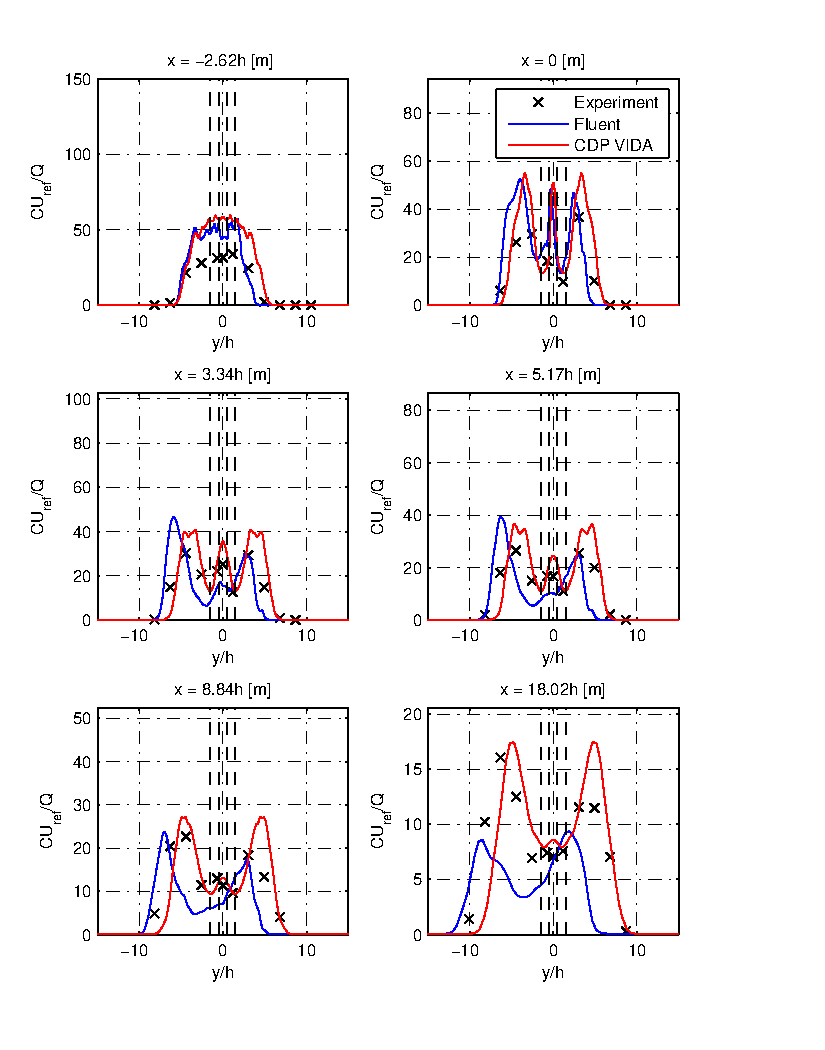
\includegraphics[width=0.7\textwidth]{figures/cHheavy.pdf}
    \caption{Time-averaged concentration with $28.8$ s of sampling at $z/H = 0.025$.
        All concentrations are scaled with the free-stream velocity and the emission rate.}
\label{fig:cHheavy}
\end{figure}
%
\newpage
Along the first two measurment lines in figure~\ref{fig:cHheavy} Fluent and CDP 
provides very similar results. And the measurement at $x = 0$ shows decent similarity 
to the experimental data as well. Further downstream Fluent fails to predict the middle 
peak which is present in both the experiment and the simulations done in CDP. The 
concentration is also consistently underestimated.
%
\begin{figure}[!h]
    \centering
    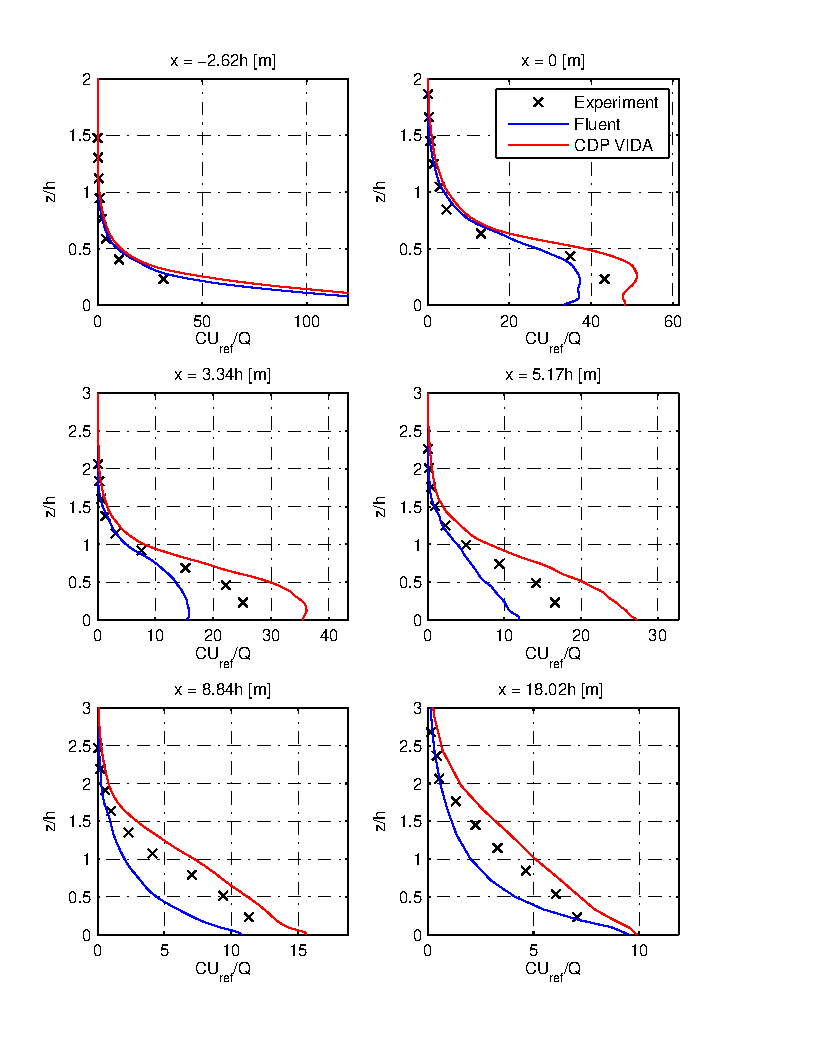
\includegraphics[width=0.8\textwidth]{figures/cVheavy.pdf}
    \caption{Time-averaged concentration with $28.8$ s of sampling at $y/H = 0$.
        All concentrations are scaled with the free-stream velocity and the emission rate.}
\label{fig:cVheavy}
\end{figure}
\newpage
%
From the data along the vertical lines plotted in figure~\ref{fig:cVheavy} Fluent consistently 
underestimates the concentration close to the wall. The slope of the profile is also very 
different from CDP and the experimental data.
%
%\begin{figure}[h]
    %\centering
    %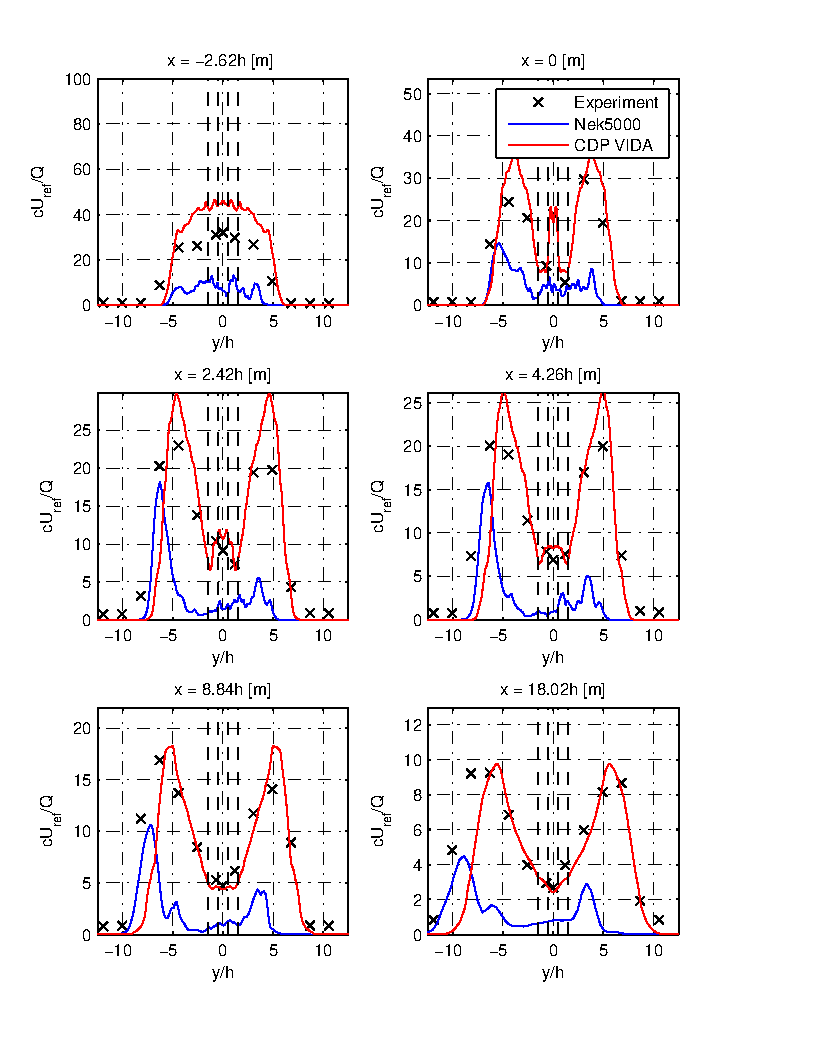
\includegraphics[width=0.8\textwidth]{figures/cfluctHheavy.pdf}
    %\caption{Time-averaged concentration with $28.8$ s of sampling at $z/H = 0.025$.
        %All concentrations are scaled with the free-stream velocity and the emission rate.}
%\label{fig:cfluctHheavy}
%\end{figure}
%

\section{Conclusion}
Fluent is compared with simulations done in CDP and experimental data. 
All simulations are done using LES\@. 
It is also experimented with different discretization schemes and the effect of an SGS model in Fluent. 
The test case is release of a neutrally buoyant gas in a turbulent boundary layer 
over an urban street canyon. 
The data used for comparison is time-averaged concentration along certain horizontal and 
vertical lines. The width and height of the plume computed in Fluent is consistent with both experimental data and simulations 
in CDP\@. There are some disagreements in the data measured close to the wall and far downstream.

The importance of the SGS model is also confirmed, although even without an SGS-model 
Fluent is able to predict a similar height and width of the plume. The shape of the 
plume is however somewhat distorted when omitting the SGS model. The increased accuracy 
achieved by increasing the degrees of freedom confirms that the model is well-functioning.

Different choices of discretization schemes can save up to 20\% of the computational 
time, but fail to provide more accurate results. The results from this case
suggests that the default settings in Fluent provide the most accurate result.

%The performance testing, analytical arguments 
%and data comparison indicates that the default settings 
%in Fluent assures a stable solution at the cost of solution accuracy and computational time.
%The results indicate that the \emph{3rd order MUSCL} scheme for the momentum equation is a better 
%choice than the default \emph{bounded central difference}. The \emph{2nd order implicit} time discretization
%can also replace the default \emph{bounded 2nd order implicit} in order to reduce
%the computational cost.  

%\input{innledning} %Dine filer
%============================================================

%===========================================================
\newpage
\bibliographystyle{plain}
\bibliography{bibliografi} %Dine referanser *.bib
\addcontentsline{toc}{section}{\numberline{}\bibname}
%=========================================================

%\newpage
%\appendix
%\section{Appendiks}

\end{document}
